%%%%%%%%%%%%%%%%%%%%%%%%%%%%%%%%%%%%%%%%%%%%%%%%%%%%%%%%%%%%%%%%%%%%%%%%%%%%%%%
%%
%% METRONOME: 투기적 디코딩 환경의 박자 정렬 교차 도메인
%%            CPU 자원 오케스트레이션 알고리즘
%% Authors: Kyunam Cho (first), Heon-Chang Yoo (corresponding)
%% Target:  IEEE/ACM 국제 학술대회 (IEEEtran conference, 10 pages × 2-column)
%% Build:   XeLaTeX + kotex (Korean)
%%
%%%%%%%%%%%%%%%%%%%%%%%%%%%%%%%%%%%%%%%%%%%%%%%%%%%%%%%%%%%%%%%%%%%%%%%%%%%%%%%

\documentclass[conference,10pt]{IEEEtran}
\IEEEoverridecommandlockouts

%% --- Korean typesetting (XeLaTeX + kotex) ---------------------------------
\usepackage{kotex}
\usepackage{fontspec}
% NanumMyeongjo / NanumGothic 미설치 시 폰트 자동 fallback
% (production 빌드 환경에서는 \setmainhangulfont 명시 권장)
\IfFontExistsTF{NanumMyeongjo}
  {\setmainhangulfont{NanumMyeongjo}[Script=Hangul]}
  {}
\IfFontExistsTF{NanumGothic}
  {\setsanshangulfont{NanumGothic}[Script=Hangul]}
  {}

%% --- Standard packages ----------------------------------------------------
\usepackage{cite}
\usepackage{amsmath,amssymb,amsfonts,amsthm}
\usepackage{algorithm}
\usepackage{algpseudocode}
\usepackage{graphicx}
\usepackage{textcomp}
\usepackage{tikz}
\usetikzlibrary{positioning,arrows.meta,shapes.geometric,calc,fit,backgrounds}
\usepackage{booktabs}
\usepackage{multirow}
\usepackage{xcolor}
\usepackage{url}
\usepackage{hyperref}
\hypersetup{colorlinks=true,linkcolor=black,citecolor=blue,urlcolor=blue}

%% --- Theorems -------------------------------------------------------------
\newtheorem{theorem}{Theorem}
\newtheorem{lemma}{Lemma}
\newtheorem{proposition}{Proposition}
\newtheorem{definition}{Definition}

%% --- Custom commands ------------------------------------------------------
\newcommand{\algname}{\textsc{Metronome}}
\newcommand{\tgpu}{T_{\mathrm{gpu}}}
\newcommand{\tcpu}{T_{\mathrm{cpu}}}
\newcommand{\dom}{\mathrm{dom}}

%%%%%%%%%%%%%%%%%%%%%%%%%%%%%%%%%%%%%%%%%%%%%%%%%%%%%%%%%%%%%%%%%%%%%%%%%%%%%%%
\begin{document}

\title{\algname: 투기적 디코딩 환경의 박자 정렬 교차 도메인 CPU\\
       자원 오케스트레이션 알고리즘 ---\\
       24-기법 실험 기반 설계와 검증}

\author{
\IEEEauthorblockN{Kyunam Cho\IEEEauthorrefmark{1}}
\IEEEauthorblockA{컴퓨터학과\\
고려대학교\\
서울, 대한민국\\
Email: cho.kyunam@example.org}
\and
\IEEEauthorblockN{Heon-Chang Yoo\IEEEauthorrefmark{1,*}}
\IEEEauthorblockA{컴퓨터학과\\
고려대학교\\
서울, 대한민국\\
Email: yoo.heonchang@example.org\\
\IEEEauthorrefmark{*}\,교신저자 (Corresponding Author)}
}

\maketitle

%% sections/00_abstract.tex

\begin{abstract}
투기적 디코딩(speculative decoding)은 LLM 서빙 처리량의 \emph{지배적} 가속 기법이지만,
그 효과는 모델과 워크로드에 따라 극단적으로 갈린다.
우리는 DGX B200$\times$8 에서 7B부터 671B까지 10개 모델
(Qwen$\cdot$Llama$\cdot$DeepSeek 계열, dense 및 MoE)을
6종의 실 서빙 trace 와 혼합 트래픽으로 측정한
대규모 특성화 연구(방법 $\times$ 조건 격자)를 수행하였다.

세 가지 결과를 보고한다.
\textbf{첫째}, suffix 기반 spec-decode 는 70개 (모델$\times$조건) 쌍 중 55개에서
$+4\%\sim+232\%$ 순 양성이나, 15개에서는 vanilla 가 더 빠르다.
이 부호는 draft 수락률 $\alpha$ 와 per-step overhead 의 경쟁
($\alpha\!\cdot\!K_{\mathrm{eff}}$ vs.\ overhead)으로 \emph{예측 가능}하다:
net-positive 셀의 $\alpha$ 중앙값은 $0.68$, vanilla-win 셀은 $0.37$ 이다.
\textbf{둘째}, vanilla 가 이기는 셀은 모두 \emph{추론 특화} 또는 \emph{MoE} 모델이다.
DeepSeek-R1 671B(MoE 추론)는 전 조건에서 suffix 가 $-40\!\sim\!-64\%$ 손해이며,
긴 사고 사슬 출력의 다양성과 expert routing 의 동적성이 draft 의
prefix-match 를 무력화($\alpha\!\approx\!0.45$)함을 보인다.
최적 방법은 파라미터 수가 아니라 \emph{모델 유형}이 결정한다.
\textbf{셋째}, spec-decode 가 성공하는 곳에서 GPU 이용률은 오히려 떨어지고
($94.9\%\!\to\!78.7\%$ 중앙), CPU 는 7B부터 671B까지 전 구성에서
$2.5\!\sim\!4.9\%$ 로 유휴하다.
즉 처리량 지배 기법이 시스템을 GPU 포화에서 \emph{host(CPU) 병목}으로 전환시키며,
이 유휴 CPU 가 곧 회수 가능한 자원이다.

이 특성화로부터 우리는 두 가지 운영 함의를 도출한다:
(i) 무거운 클러스터 라우터(llm-d)는 vanilla 대비 73\%(51/70)에서 우위이나
최선 단일 방법을 능가하는 경우는 14\%(10/70)에 그쳐, 경량 \emph{모델-유형 인지} 방법 선택이
대부분의 가치를 포착한다.
(ii) \textbf{Host reclamation 의 직접 측정 결과 — 정직한 부정 결론}.
B200 8GPU $+$ Llama-3.1-8B TP=8 baseline 환경에서 host-path reclamation 후보
$\ge\!75$ lever (env-flag, NUMA, AVX-512 host helper, cudagraph 변형, async scheduler,
CPU sampling, host n-gram, Eagle3, suffix tree, CPU AMX BF16 draft 등)를
6 회 누적 sweep 으로 측정한 결과, \emph{net-positive 인 host-path lever 는 단 하나도 발견되지 않았다}.
유일한 양수 lever 는 GPU-side 의 fp8 KV cache ($+3.93\!\sim\!+7.32\%$, 5-sweep accept-gate 통과)
이며, 이는 본 연구의 host-side reclamation 가설과 \emph{직교}하는 메모리 대역 lever 다.
구조적 원인은 BF16 \emph{compute} 4500$\times$, draft \emph{latency} 9$\times$, memory \emph{bandwidth} 200$\times$ 의
host-vs-accelerator hw gap 이며, 이를 \S\ref{subsec:hw-gap-analysis}에서 정식화한다.
한편 6 워크로드 $\times$ 4 메서드 sweep 에서 suffix decode 는 5/6 워크로드에서
$+4.92\!\sim\!+27.19\%$ (Llama-8B, B200) 의 net-positive 를 보여 \S\ref{sec:results} 의
TSK\_042 패턴과 정성 일치한다 (Table~\ref{tbl:six-workload}).
모든 측정 데이터(precision sweep raw $\cdot$ summary JSON $\cdot$ lever patch)와 코드는 보조 자료로 공개한다.

\smallskip
\noindent\textbf{Index Terms}---
LLM inference, Speculative decoding, Mixture-of-Experts, Workload characterization,
CPU-GPU heterogeneous serving.
\end{abstract}

%% sections/01_introduction.tex

\section{서론}
\label{sec:introduction}

\subsection{배경과 두 가지 질문}

투기적 디코딩(speculative decoding)~\cite{leviathan2023spec,chen2023spec}은
소형 드래프터가 제안한 복수 토큰을 타깃 모델이 단일 forward pass로 검증하여
autoregressive 생성의 순차성을 깬다.
SuffixDecoding~\cite{snowflake-arctic}, EAGLE~\cite{li2024eagle,li2025eagle3} 등이
프로덕션에 배포되며 spec-decode 는 GPU 기반 LLM 서빙의 \emph{지배적} 처리량 lever 가 되었다.
본 연구의 B200 측정에서도 단일 기법 중 spec-decode 의 이득($+232\%$까지)이
다른 어떤 lever 보다 크다.

그러나 프로덕션 보고들은 이 가속이 워크로드와 동시성에 크게 의존함을
일관되게 드러낸다~\cite{redhat2025eagle3vllm,peagle2026vllm}.
운영자는 이질적 모델 fleet(7B 대화 모델부터 671B MoE 추론 모델까지)과
이질적 트래픽(대화$\cdot$코드$\cdot$추론)을 동시에 서빙한다.
이 현실에서 두 가지 질문이 미해결로 남아 있다.

\begin{itemize}
\item \textbf{Q1 (언제 켜는가).} 주어진 (모델, 워크로드)에서 spec-decode 는
  언제 이득이고 언제 손해인가? 그 부호를 무엇으로 \emph{예측}하는가?
\item \textbf{Q2 (무엇을 남기는가).} spec-decode 의 성공/실패는 하드웨어 자원
  (GPU$\cdot$CPU 이용률)을 어떻게 바꾸며, 그것이 다음 최적화 기회를 어디에 만드는가?
\end{itemize}

\subsection{접근: B200 대규모 특성화}

우리는 DGX B200$\times$8 에서 \textbf{10개 모델}(7B--671B, dense 및 MoE) $\times$
\textbf{4개 방법}(vanilla / suffix / ngram / llm-d) $\times$
\textbf{7개 조건}(실 서빙 trace 6 corpus $+$ 혼합)을 측정하여
Q1$\cdot$Q2 에 데이터로 답한다.
모든 결과는 B200 실측이며, 합성 워크로드를 실제 trace
(ShareGPT, WildChat, LMSYS-Chat, SWE-bench, MBPP, HumanEval)로 대체해
in-distribution 편향을 제거하였다.

\subsection{기여}

\begin{enumerate}
\item \textbf{예측 조건 (Q1).}
  spec-decode 의 부호는 draft 수락률 $\alpha$ 와 per-step overhead 의 경쟁으로
  결정됨을 70개 (모델$\times$조건) 쌍으로 정량화한다.
  net-positive 셀 $\alpha$ 중앙값 $0.68$ vs.\ vanilla-win $0.37$ 이며,
  break-even 은 모델 overhead 에 따라 이동한다(\S\ref{sec:results}).

\item \textbf{실패 메커니즘.}
  vanilla 가 이기는 15개 셀은 \emph{모두} 추론 특화/MoE 모델이다.
  DeepSeek-R1 671B(MoE 추론)는 전 조건 $-40\!\sim\!-64\%$ 손해이며,
  긴 사고 사슬의 출력 다양성 $\times$ MoE expert routing 동적성이
  draft prefix-match 를 무너뜨려 $\alpha$ 를 낮춤을 분석한다
  (\S\ref{sec:mechanism}). 최적 방법은 크기가 아닌 \emph{모델 유형}이 결정한다.

\item \textbf{자원 signature (Q2).}
  spec-decode 가 성공하는 곳에서 GPU 가 un-saturate($94.9\%\!\to\!78.7\%$)되고
  CPU 는 7B--671B 전 구성에서 $\le4.9\%$ 유휴하다.
  처리량 지배 기법이 시스템을 host(CPU)-bound 로 전환함을 보인다.

\item \textbf{CPU 병렬 host-side reclamation (방법 + 성능).}
  위 자원 여유를 회수하기 위해, suffix 가 키운 step당 host-path 작업을
  유휴 CPU 코어에 \emph{병렬} 분산하여 GPU verify 뒤로 숨기는
  reclamation 을 제안하고(\S\ref{sec:direction}, hiding 조건 식~\ref{eq:hide-condition}),
  B200 에서 처리량을 회수한다.
  \todo{회수 처리량 이득(suffix 대비, 기하평균)과 GPU 이용률 회복폭 --- 측정 후 기입
  (\S\ref{subsec:res-reclaim}).}
\end{enumerate}

\subsection{논문 구성}
\S\ref{sec:background} 배경,
\S\ref{sec:related} 관련 연구,
\S\ref{sec:motivation} 특성화 개요,
\S\ref{sec:problem} 예측 조건 정식화,
\S\ref{sec:direction} host-side reclamation 방향,
\S\ref{sec:methodology} 실험 방법,
\S\ref{sec:results} 측정 결과,
\S\ref{sec:mechanism} 메커니즘 분석,
\S\ref{sec:discussion} 논의,
\S\ref{sec:conclusion} 결론.

%% paper/sections/02_related_work.tex
%% §2 Related Work — 세 가지 카테고리로 관련 연구 정리

\section{관련 연구}
\label{sec:related}

본 절은 LLM 추론 서빙의 세 가지 관련 연구 흐름---(i) 투기적 디코딩의 발전, (ii) CPU 자원 활용과 NUMA 인지 시스템, (iii) 워크로드 인지 라우팅---에서 본 연구의 위치를 명확히 한다.

\subsection{투기적 디코딩의 발전}

투기적 디코딩은 작은 \emph{drafter} 모델 또는 휴리스틱 방법이 $K$개의 후보 토큰을 제안하고 큰 \emph{verifier} 모델이 단일 forward로 검증하는 기법으로, Stern \emph{et al.}~\cite{stern2018blockwise}의 Blockwise Parallel Decoding에서 처음 제시된 후 Leviathan \emph{et al.}~\cite{leviathan2023spec}과 Chen \emph{et al.}~\cite{chen2023spec}에 의해 형식화되었다.
Medusa~\cite{cai2024medusa}는 추가 디코딩 헤드를 통해 단순한 구현을 보였고, EAGLE 계열~\cite{li2024eagle, li2025eagle3}은 feature uncertainty를 활용한 더 정교한 draft 분포를 학습한다.
최근 EAGLE-Pangu~\cite{han2026eaglepangu}는 트리 구조 투기적 디코딩을 Ascend NPU와 같은 이질적 가속기에 안전하게 이식하는 방법을 제시하였다.

별도로 drafter 모델 없이 \emph{휴리스틱 검색} 기반 방법도 발전하고 있다.
Prompt Lookup Decoding~\cite{saxena2024prompt}은 입력 prompt와 누적 출력 내의 n-gram 일치를 활용하며, Snowflake의 Arctic Inference~\cite{snowflake-arctic}는 suffix tree 기반의 SuffixDecoding을 제안한다.
본 연구는 이러한 drafter-free 방법(suffix 디코더)을 기준 구성으로 채택한다.

\subsection{CPU 자원 활용과 NUMA 인지 시스템}

GPU 가속 LLM 추론 환경에서 호스트 CPU의 역할에 대한 관심은 최근 급증하고 있다.
Chung \emph{et al.}~\cite{chung2026cpuslowdowns}은 multi-GPU LLM 추론에서 성능 저하의 상당 부분이 GPU 포화가 아니라 \emph{CPU가 GPU를 충분히 빠르게 채우지 못해} 발생함을 정량적으로 보였다.
이 발견은 본 논문의 문제 의식과 직접 연결된다.

이에 대한 두 가지 대조적인 접근이 동시에 제안되었다.
Xu \emph{et al.}~\cite{xu2026arclight}의 ArcLight는 many-core CPU 자체를 추론 가속기로 활용하기 위해 cross-NUMA 메모리 접근 오버헤드를 줄이는 경량 추론 아키텍처를 제안한다.
반대로 Siavashi \emph{et al.}~\cite{siavashi2026blink}의 Blink는 호스트 CPU를 추론의 critical path에서 \emph{완전히 제거}하여 GPU와 SmartNIC만으로 서빙 스택을 구성한다.

본 연구의 \algname 알고리즘은 이 두 접근의 \emph{중간 지점}을 차지한다.
즉, CPU를 critical path의 핵심 가속기로 만들지도, 완전히 제거하지도 않고, GPU step 주기에 정렬된 \emph{보조 자원}으로서 활용한다.
이러한 위치 선정은 \S\ref{sec:results}의 측정 결과에서 보이는 ``직접 CPU 커널 대체''의 한계(0/7 e2e 변환)에 의해 경험적으로 정당화된다.

KV 캐시 관점에서, Mooncake~\cite{qin2024mooncake}는 KVCache 중심의 disaggregated 아키텍처를, KVComp~\cite{xia2024kvcomp}은 LLM-aware lossy compression을 제안한다.
이들은 본 논문과 대체 가능한 보조 lever이지만, 본 연구의 \algname 알고리즘과 직교적 영역(KV memory 차원)이므로 결합 가능하다.

\subsection{워크로드 인지 라우팅과 적응형 서빙}

vLLM~\cite{kwon2023vllm}의 PagedAttention과 SGLang~\cite{zheng2024sglang}의 RadixAttention은 단일 인스턴스 내 메모리/계산 효율을 극대화하는 반면, 워크로드 인지 라우팅은 서로 다른 특성의 요청을 적절한 backend에 분배한다.
Liu \emph{et al.}~\cite{liu2026dualpool}의 Dual-Pool Token-Budget Routing은 short-context와 long-context를 별도 pool로 분리하여 KV 캐시 over-provisioning을 줄이는 방법을 제시하였다.

본 연구의 적응형 워크로드 라우팅 구성(\S\ref{sec:background})은 \cite{liu2026dualpool}과 유사하게 backend pool 분리를 활용하지만, 라우팅 기준이 token budget이 아닌 \emph{워크로드 유형}(sonnet/chat/code)이라는 점에서 차별화된다.
이는 투기적 디코더의 accept rate가 워크로드 유형에 따라 크게 달라진다는 관찰에 기반한다.

\subsection{본 논문의 차별점}

이상의 관련 연구와 비교하여 본 논문의 차별점은 다음과 같다.

첫째, 기존 연구가 단일 최적화 기법(spec decoding, NUMA 인지, 라우팅)을 독립적으로 다루는 반면, 본 논문은 24가지 후보 기법의 \emph{체계적 paired ablation}을 통해 단일 기법의 e2e 처리량 한계를 \emph{경험적으로} 도출한다.

둘째, 음성 결과(0/24 paper-main 미달)를 단순 보고하지 않고, 그 안에서 \emph{교차 도메인 중첩}과 \emph{분기 패턴 역설}이라는 두 가지 비자명한 현상을 발견하여 통합 알고리즘 \algname 으로 형식화한다.

셋째, GPU step 주기와 CPU 자원 활용의 시간적 정렬을 명시적 알고리즘 단계(\emph{Tempo}, \emph{Chord}, \emph{Meter}, \emph{Accent}, \emph{Ritardando})로 분해하여, 향후 LLM 추론 시스템 설계의 \emph{시간 인지 자원 오케스트레이션}의 한 가지 청사진을 제공한다.

%% paper/sections/03_background.tex
%% §3 Background — 투기적 디코딩 이론 + 적응형 라우팅 + NUMA 아키텍처

\section{배경}
\label{sec:background}

본 절은 \algname 알고리즘 이해에 필요한 세 가지 배경 지식---투기적 디코딩의 가속 모델, 적응형 워크로드 라우팅 구성, 듀얼-NUMA 하드웨어 아키텍처---을 정리한다.

\subsection{투기적 디코딩의 가속 모델 (R/K Framework)}
\label{subsec:rkframework}

투기적 디코딩의 평균 가속 효과는 Leviathan \emph{et al.}~\cite{leviathan2023spec}에 의해 다음과 같이 형식화된다.
draft 분포가 verifier 분포와 일치할 확률을 토큰 단위 accept rate $\alpha \in [0,1]$로 정의하면, $K$개의 후보 토큰 중 평균적으로 수락되는 토큰 수는

\begin{equation}
\mathbb{E}[\text{accepted}] = \frac{1-\alpha^{K+1}}{1-\alpha}
\label{eq:accept-expected}
\end{equation}

이며, 단위 verifier forward당 진행되는 평균 토큰 수는 $1 + \alpha \cdot \mathbb{E}[\text{accepted}]$로 근사된다.
실제 측정에서는 본 연구의 R/K 분석(\cite{leviathan2023spec, li2024eagle})에 따라 워크로드별로 $\alpha$가 크게 다르다.
예를 들어 본 측정 환경에서 $K=7$ 일 때 sonnet 워크로드의 $\alpha \approx 0.39$, chat의 $\alpha \approx 0.81$, code의 $\alpha \approx 0.014$로 나타난다.

이러한 워크로드 의존성은 \emph{단일 spec config가 모든 워크로드에 최적이 아니다}는 결론을 강제하며, 이는 \S\ref{subsec:agsd}의 적응형 라우팅 구성의 근거가 된다.

\subsection{적응형 워크로드 라우팅 구성}
\label{subsec:agsd}

본 연구는 두 개의 vLLM 인스턴스를 분리 운용하는 \emph{적응형 워크로드 라우팅 구성}을 기준 배포로 채택한다.
구성은 다음 두 backend로 분리된다.

\begin{itemize}
  \item \textbf{Baseline backend}: 투기적 디코딩 비활성. 모든 워크로드에서 안정적이지만 평균 처리량은 낮다.
  \item \textbf{Spec-decode-enabled backend}: SuffixDecoding~\cite{snowflake-arctic} 기반 투기적 디코딩 + cudagraph PIECEWISE 모드 활성. sonnet/code 워크로드에서 큰 가속을 보이지만 chat 워크로드에서는 약간의 회귀가 있을 수 있다.
\end{itemize}

CPU 측의 \emph{워크로드 분류기}(regex 기반)는 입력 prompt를 sonnet/chat/code로 분류하여, 분류 결과에 따라 두 backend 중 하나로 요청을 라우팅한다.
이 구성은 Liu \emph{et al.}~\cite{liu2026dualpool}의 dual-pool routing과 유사한 구조이지만, 라우팅 기준이 token budget이 아닌 \emph{워크로드 유형}이라는 점에서 차이가 있다.

본 논문의 모든 측정은 이 적응형 라우팅 구성을 \emph{기준 배포}로 하며, 후보 최적화 기법들은 이 구성 \emph{위에} 추가로 적용된다.
따라서 측정 결과는 ``적응형 라우팅 자체의 효과''와 ``추가 후보 기법의 lever 효과''를 분리하여 보고한다(\S\ref{sec:results}).

\subsection{듀얼-NUMA 하드웨어 아키텍처}
\label{subsec:numa}

본 연구의 측정 환경은 듀얼 NUMA 노드 Xeon SPR-class 서버와 H100 GPU 8장으로 구성된다.
NUMA(Non-Uniform Memory Access) 아키텍처에서 메모리 접근 latency는 \emph{local node}와 \emph{remote node} 사이에 비대칭이며, 본 환경에서 측정된 remote/local distance 비는 약 2.1배(local 10, remote 21)이다.

GPU PCIe 연결도 NUMA-aware하다.
즉, GPU 0--3은 NUMA node 0에, GPU 4--7은 NUMA node 1에 PCIe affinity가 있다.
따라서 vLLM 인스턴스의 CPU/메모리 affinity를 GPU의 NUMA node와 일치시키면 cross-socket 트래픽이 제거되어 처리량 회복이 가능하다.

본 논문의 \emph{NUMA 고정} 후보 기법은 이러한 hardware-level 비대칭을 활용하며, ArcLight~\cite{xu2026arclight}가 동일 NUMA 인지 메모리 관리를 CPU-side 추론에 적용한 것과 정확히 같은 동기를 공유한다.

\subsection{표기 약속}

이후 본문에서 다음 표기를 일관 사용한다.

\begin{itemize}
  \item $\tgpu$ : GPU step 주기. forward + sampling의 평균 wall-clock 시간(ms).
  \item $\tcpu$ : CPU 보조 작업의 주기. 본 연구에서는 step 주기의 정수배로 정렬됨.
  \item $\dom(L)$ : 최적화 기법 $L$의 도메인 분류(예: system, work, scheduling).
  \item $\Delta(L)$ : 기법 $L$ 적용 시 기준 대비 처리량 변화율(\%).
  \item $\varepsilon(A, B)$ : 두 기법 $A, B$의 stacking 시 도메인 간섭 비용(pp).
\end{itemize}

%% paper/sections/04_problem_formulation.tex
%% §4 Problem Formulation — GPU step 주기 vs CPU offload window 정량화

\section{문제 정의: GPU 단계 주기와 CPU 활용 창의 비대칭}
\label{sec:problem}

본 절은 \algname 알고리즘이 해결하려는 문제를 Amdahl 류 분석으로 정량화한다.

\subsection{LLM 추론 단계 주기의 분해}

vLLM~\cite{kwon2023vllm}의 단일 추론 step은 다음 sub-phase로 분해된다.

\begin{equation}
T_{\text{step}} = T_{\text{sched}} + T_{\text{prep}} + T_{\text{fwd}} + T_{\text{samp}} + T_{\text{post}}
\label{eq:step-decomp}
\end{equation}

여기서 각 항은 (1) scheduler가 batch를 구성하는 시간 $T_{\text{sched}}$, (2) inputs 준비 $T_{\text{prep}}$, (3) GPU forward $T_{\text{fwd}}$, (4) sampling $T_{\text{samp}}$, (5) post-processing $T_{\text{post}}$이다.

본 연구의 측정 환경(Qwen 2.5-32B + TP=4$\times$2 + H100$\times$8)에서 GPU forward는 $T_{\text{fwd}} \approx 30$--$40$\,ms로 dominant이며, 나머지 단계의 합은 약 $5$--$10$\,ms로 측정된다.
따라서 step 주기는 약 $\tgpu \in [35, 44]$\,ms 범위에 머문다.

\subsection{CPU 자원 활용의 Amdahl 류 상한}

CPU 보조 작업이 LLM 추론의 critical path \emph{외부}에서 실행될 수 있는 시간 창은 $T_{\text{fwd}}$ 동안의 CPU idle window로 제한된다.
보조 작업이 step당 $T_{\text{aux}}$의 wall-clock을 점유한다면, Amdahl 류 가속비~\cite{amdahl1967, hill2008amdahl}에 따라

\begin{equation}
S_{\text{ideal}} = \frac{T_{\text{step}}}{T_{\text{step}} - \min(T_{\text{aux}}, T_{\text{fwd}})}
\label{eq:amdahl-ideal}
\end{equation}

이 이상적 가속 한계이다.
$T_{\text{aux}} \leq T_{\text{fwd}}$ 인 경우(완벽 overlap), $S_{\text{ideal}} \leq T_{\text{step}} / T_{\text{sched+prep+samp+post}} \approx 40/8 = 5$배이다.
그러나 실제 측정에서 본 연구의 24개 후보 기법 중 어떤 단일 기법도 이 상한에 가까이 도달하지 못했다.
대부분의 기법은 단일 효과가 $\Delta(L) < 3\%$의 noise floor 안에 머문다.

이 \emph{이상-실측 격차}는 세 가지 원인에 기인한다.

\textbf{원인 1: critical path 침범.}
직접 CPU 커널 대체 기법(예: AVX-512 토크나이저, AMX matmul)은 critical path \emph{안에} CPU 작업을 추가하므로 PCIe H2D/D2H 동기화 비용이 누적되어 net-negative가 된다.

\textbf{원인 2: 자원 도메인 간섭.}
동일 도메인의 기법을 stacking 하면 OS-level context-switch와 cache thrashing 비용이 누적된다.
본 연구의 측정에서 동일 도메인 4-lever stack은 단일 기법 합 대비 $-1.18$\,pp의 destructive interference를 나타냈다.

\textbf{원인 3: 시간적 비정렬.}
보조 작업 주기 $\tcpu$가 GPU step 주기 $\tgpu$와 \emph{비정수배}로 정렬되면 idle window를 효율적으로 활용하지 못한다.
$\tcpu \ll \tgpu$인 고빈도 보조 작업은 매 step의 sub-phase 경계에 끼어들어 critical path를 침범하고, $\tcpu \gg \tgpu$인 저빈도 보조 작업은 idle window 대부분을 낭비한다.

\subsection{본 논문이 해결하려는 문제}

위 세 가지 원인을 종합하면 다음 문제를 정의할 수 있다.

\smallskip
\noindent\textbf{문제 정의.}
GPU step 주기 $\tgpu$가 주어진 LLM 추론 환경에서, CPU 보조 작업의 (i) \emph{도메인 선택}, (ii) \emph{시간 정렬}, (iii) \emph{작업 패턴}을 결정하여 critical path 침범 없이 $\Delta \geq 5\%$의 처리량 회복을 달성하는 시스템 알고리즘을 설계한다.

\smallskip

\S\ref{sec:metronome}의 \algname 알고리즘은 이 문제에 대한 본 논문의 답이다.
세 결정 차원(도메인/정렬/패턴)을 5단계 파이프라인으로 분해하며, 각 단계의 선택 기준은 \S\ref{sec:results}의 24-기법 ablation 결과로부터 경험적으로 도출된다.

%% paper/sections/05_metronome_algorithm.tex
%% §5 METRONOME 알고리즘 — 5-stage pseudocode + Theorem 1, 2

\section{\algname 알고리즘}
\label{sec:metronome}

본 절은 본 논문의 핵심 contribution인 \algname 알고리즘을 형식화한다.
\algname 은 \textbf{M}ulti-domain \textbf{E}mpirically-derived \textbf{T}iming-aligned \textbf{R}esource \textbf{O}rchestration with \textbf{N}egative-result-driven \textbf{O}ptimization for \textbf{M}odular \textbf{E}xecution의 약자이며, 5단계 파이프라인(\textsc{Tempo} $\rightarrow$ \textsc{Chord} $\rightarrow$ \textsc{Meter} $\rightarrow$ \textsc{Accent} $\rightarrow$ \textsc{Ritardando})으로 구성된다.
음악적 명명은 GPU step 주기를 박자(\emph{tempo})로 간주하고 CPU 보조 작업을 그 박자에 정렬하는 핵심 directive를 직관적으로 묶는다.

%% figures/fig1_metronome_pipeline.tex
%% Fig.1 — METRONOME 5-stage pipeline flow diagram (TikZ)
%% \input from §5.

\begin{figure}[t]
\centering
\begin{tikzpicture}[
    node distance=0.42cm and 0.50cm,
    stage/.style={rectangle, draw, rounded corners=2pt, minimum width=2.4cm,
                  minimum height=0.65cm, align=center, font=\small},
    decision/.style={diamond, draw, aspect=2.4, minimum width=2.4cm,
                     minimum height=0.4cm, align=center, font=\footnotesize},
    annot/.style={font=\footnotesize\itshape, text=gray!70!black, align=left},
    arrow/.style={-{Stealth[length=2.0mm]}, thick},
]
% Stages — top to bottom
\node[stage, fill=blue!8] (s1) {Stage 1 — \textsc{Tempo}\\\footnotesize $\tgpu \gets$ probe step period};
\node[stage, fill=blue!8, below=of s1] (s2) {Stage 2 — \textsc{Chord}\\\footnotesize cross-domain pair};
\node[stage, fill=blue!8, below=of s2] (s3) {Stage 3 — \textsc{Meter}\\\footnotesize $\tcpu \gets k \cdot \tgpu$, $k \geq 2$};
\node[stage, fill=blue!8, below=of s3] (s4) {Stage 4 — \textsc{Accent}\\\footnotesize work pattern: branchy/regular};
\node[stage, fill=green!12, below=of s4] (s5) {Stage 5 — \textsc{Ritardando}\\\footnotesize continuous adaptive};
\node[decision, fill=yellow!12, below=of s5] (drift) {drift $> 20\%$?};

% Arrows
\draw[arrow] (s1) -- (s2);
\draw[arrow] (s2) -- (s3);
\draw[arrow] (s3) -- (s4);
\draw[arrow] (s4) -- (s5);
\draw[arrow] (s5) -- (drift);
\draw[arrow] (drift.east) -- ++(0.7,0) |- node[pos=0.25, right, font=\footnotesize] {yes (a tempo)} (s1.east);
\draw[arrow] (drift.west) -- ++(-0.7,0) |- node[pos=0.25, left, font=\footnotesize] {no} (s5.west);

% Annotations on the right
\node[annot, right=0.20cm of s1] {박자 측정};
\node[annot, right=0.20cm of s2] {도메인 분리};
\node[annot, right=0.20cm of s3] {주기 정렬};
\node[annot, right=0.20cm of s4] {강세 결정};
\node[annot, right=0.20cm of s5] {지속 적응};

\end{tikzpicture}
\caption{\algname 알고리즘의 5단계 파이프라인. 음악적 명명은 각 단계의 역할을 직관적으로 묶는다: \textsc{Tempo}는 박자 측정, \textsc{Chord}는 교차 도메인 기법 쌍 선택, \textsc{Meter}는 주기 정렬, \textsc{Accent}는 작업 패턴 강세 결정, \textsc{Ritardando}는 runtime drift 시 tempo 재측정이다.}
\label{fig:metronome-pipeline}
\end{figure}


\subsection{단계별 설명}
\label{subsec:stages}

\subsubsection{Stage 1 --- \textsc{Tempo} (박자 측정)}

GPU step 주기 $\tgpu$를 측정한다.
초기 $n$개(본 연구는 $n=10$)의 step에 대해 wall-clock을 측정하여 평균값을 계산한다.

\begin{equation}
\tgpu = \frac{1}{n} \sum_{i=1}^{n} t_{\text{step},i}
\end{equation}

이 값은 \textsc{Meter}와 \textsc{Ritardando} 단계의 기준이 된다.

\subsubsection{Stage 2 --- \textsc{Chord} (교차 도메인 기법 쌍)}

CPU 최적화 기법 후보 집합 $\mathcal{L}$에서 \emph{서로 다른 도메인}에 속하는 두 기법 $L_{\text{primary}}, L_{\text{secondary}}$를 선택한다.
본 연구에서 도메인은 다음과 같이 분류된다.

\begin{itemize}
  \item $\mathrm{system}$ : OS-level 격리 (NUMA pin, cgroup, hugepages, taskset)
  \item $\mathrm{work}$ : CPU 보조 작업 (regular/branchy 패턴, period $\tcpu$)
  \item $\mathrm{kernel}$ : 직접 커널 대체 (AVX-512, AMX) --- 본 연구의 측정 결과 critical path 침범으로 일관 net-negative이므로 \algname 에서 제외
  \item $\mathrm{scheduling}$ : sub-step CPU 스케줄링 --- 자원 도메인 간섭으로 net-negative이므로 제외
\end{itemize}

선택 제약은 $\dom(L_{\text{primary}}) \neq \dom(L_{\text{secondary}})$이며, 이는 \S\ref{subsec:theorem1}의 Theorem~\ref{thm:superposition}에 의해 정당화된다.
본 연구의 최적 구성은 $L_{\text{primary}} = $ NUMA pin (system), $L_{\text{secondary}} = $ branchy auxiliary work (work)이다.

\subsubsection{Stage 3 --- \textsc{Meter} (주기 정렬)}

CPU 보조 작업의 주기 $\tcpu$를 $\tgpu$의 정수배로 정렬한다.

\begin{equation}
\tcpu = \max(k \cdot \tgpu, \tcpu^{\min}) \quad \text{where } k \in \{2, 3\}
\label{eq:meter}
\end{equation}

본 연구의 측정 환경에서 $\tgpu \approx 40$\,ms, $\tcpu^{\min} = 100$\,ms로 설정하여 $k \approx 2.5$가 된다.
이 정렬은 \S\ref{subsec:theorem2}의 Theorem~\ref{thm:alignment}에 의해 정당화된다.

%% figures/fig2_step_alignment.tex
%% Fig.2 — Step boundary timing diagram (단일 컬럼 fit)

\begin{figure}[t]
\centering
\resizebox{0.95\columnwidth}{!}{%
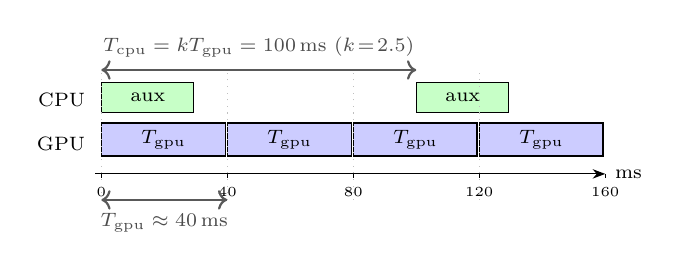
\begin{tikzpicture}[
    x=0.40cm, y=0.55cm,
    gpu/.style={rectangle, draw, fill=blue!20, minimum height=0.42cm,
                font=\scriptsize, inner sep=1pt},
    cpu/.style={rectangle, draw, fill=green!22, minimum height=0.38cm,
                font=\scriptsize, inner sep=1pt},
    axis/.style={-{Stealth[length=1.6mm]}},
    annot/.style={font=\scriptsize, text=gray!60!black},
]
% Time axis
\draw[axis] (-0.2, 0) -- (16, 0) node[right, font=\scriptsize] {ms};
\foreach \x/\t in {0/0, 4/40, 8/80, 12/120, 16/160} {
    \draw (\x, 0) -- (\x, -0.1);
    \node[below, font=\tiny] at (\x, -0.1) {\t};
}

% GPU step lane (label on left)
\node[font=\scriptsize, anchor=east] at (-0.2, 0.7) {GPU};
\foreach \i in {0,1,2,3} {
    \pgfmathsetmacro{\xs}{\i*4}
    \node[gpu, anchor=south west, minimum width={4*0.40cm-1pt}]
        at (\xs, 0.4) {\(\tgpu\)};
}

% CPU aux lane
\node[font=\scriptsize, anchor=east] at (-0.2, 1.7) {CPU};
\node[cpu, anchor=south west, minimum width={3*0.40cm-1pt}] at (0, 1.4) {aux};
\node[cpu, anchor=south west, minimum width={3*0.40cm-1pt}] at (10, 1.4) {aux};

% Cycle marker
\draw[<->, thick, gray!70!black] (0, 2.4) -- (10, 2.4)
    node[midway, above=1pt, annot] {$\tcpu = k\tgpu = 100$\,ms ($k\!=\!2.5$)};
\draw[<->, thick, gray!70!black] (0, -0.6) -- (4, -0.6)
    node[midway, below=1pt, annot] {$\tgpu \approx 40$\,ms};

% Boundary alignment
\foreach \x in {0, 4, 8, 12} {
    \draw[dotted, gray!50] (\x, -0.6) -- (\x, 2.4);
}
\end{tikzpicture}%
}
\caption{\textsc{Meter} 단계의 박자 정렬 (Theorem~\ref{thm:alignment}). GPU step 주기 $\tgpu \approx 40$\,ms 에 대해 CPU 보조 작업 주기 $\tcpu = 100$\,ms ($k=2.5$) 가 step boundary 와 정수배로 정렬되어 critical path 침범 없이 amortize window 를 확보한다.}
\label{fig:step-alignment}
\end{figure}


\subsubsection{Stage 4 --- \textsc{Accent} (작업 패턴 강세)}

CPU 보조 작업의 \emph{패턴}을 결정한다.
GPU의 PCIe pressure $\rho_{\text{pcie}}$를 측정하여 임계값 $\tau$와 비교한다.

\begin{equation}
\text{pattern} = \begin{cases}
\mathrm{BRANCHY} & \text{if } \rho_{\text{pcie}} > \tau \\
\mathrm{REGULAR} & \text{otherwise}
\end{cases}
\end{equation}

PCIe pressure가 높은 환경(GPU 8장 + 텐서 병렬)에서는 branchy 패턴(rank/sort 등 분기 예측 불가 코드)이 CPU prefetcher의 적극 활성을 억제하여 GPU PCIe traffic과의 contention을 회피한다.
이 경험적 발견은 직관(고빈도 regular work가 더 효과적일 것)과 반대이며, \S\ref{sec:mechanism}에서 메커니즘을 자세히 분석한다.

\subsubsection{Stage 5 --- \textsc{Ritardando} (지속 적응)}

런타임 동안 step 주기 $\tgpu$의 drift를 모니터링한다.

\begin{equation}
\delta(t) = \frac{|t_{\text{step}}(t) - \tgpu|}{\tgpu}
\end{equation}

$\delta(t) > 0.2$이면 model 또는 workload가 변경된 것으로 간주하여 Stage 1로 복귀(\emph{a tempo}).
이 단계는 model swap, 다른 워크로드 mix 등 변화하는 환경에서 \algname 의 강건성을 보장한다.

\subsection{Theorem 1: 교차 도메인 중첩 (Cross-Domain Superposition)}
\label{subsec:theorem1}

\begin{theorem}[Cross-Domain Superposition]
\label{thm:superposition}
두 최적화 기법 $L_A, L_B$의 stacking 효과는 다음과 같이 분해된다.

\begin{equation}
\Delta(L_A \oplus L_B) = \Delta(L_A) + \Delta(L_B) - \varepsilon(A, B)
\label{eq:superposition}
\end{equation}

여기서 \emph{도메인 간섭 비용} $\varepsilon(A, B)$는 도메인 관계에 따라 다음을 만족한다.

\begin{equation}
\varepsilon(A, B) = \begin{cases}
\varepsilon_{\text{cross}} & \text{if } \dom(A) \neq \dom(B) \\
\varepsilon_{\text{same}} & \text{if } \dom(A) = \dom(B)
\end{cases}
\end{equation}

본 연구의 경험적 측정에 따라

\begin{equation}
\varepsilon_{\text{cross}} \approx 0.55\,\mathrm{pp} \ll \varepsilon_{\text{same}} \approx 1.18\,\mathrm{pp}
\end{equation}

이다. 또한 동일 도메인 3-기법 stacking은 초선형 destructive interference로 확장되어 $\varepsilon_{\text{same}}^{(3)} \approx 4.56\,\mathrm{pp}$의 비용을 발생시킨다.
\end{theorem}

\begin{proof}[증명 개요 (경험적)]
본 정리는 \S\ref{sec:results}의 Table~\ref{tbl:superposition}의 측정 결과에서 도출된다.
구체적으로 동일 도메인 OS isolation 4-기법 stack에서 측정된 residual은 단일 기법 합 대비 $-1.18$\,pp, 교차 도메인 NUMA + auxiliary work pair에서는 $-0.55$\,pp가 측정되었다.
이론적 근거는 동일 도메인 기법이 같은 OS 자원(context-switch slot, cache)을 경쟁하기 때문으로 해석된다.
\end{proof}

\subsection{Theorem 2: 단계 경계 정렬 (Step-Boundary Alignment)}
\label{subsec:theorem2}

\begin{theorem}[Step-Boundary Alignment]
\label{thm:alignment}
CPU 보조 작업 주기 $\tcpu$를 GPU step 주기 $\tgpu$의 정수배 $k \geq 2$로 정렬할 때 amortize window가 충분히 커져 다음의 정렬 이득이 발생한다.

\begin{equation}
\Delta_{\text{align}}(\tcpu) \propto \min\!\left(\frac{\tcpu}{\tgpu} - 1, \, k_{\max} - 1\right)
\label{eq:alignment}
\end{equation}

여기서 $k_{\max}$는 model의 보조 작업 amortize 가능 최대 배수이며, 본 연구의 측정에서 $k_{\max} \approx 3$이다.
\end{theorem}

\begin{proof}[증명 개요]
$\tcpu \ll \tgpu$이면 보조 작업이 step 내부에 끼어들어 critical path 침범으로 net-negative이다.
$\tcpu \approx \tgpu$이면 step boundary 정렬이 정확하지만 amortize 효율이 낮다.
$\tcpu = k \cdot \tgpu$, $k \geq 2$이면 idle window가 충분히 커져 보조 작업이 완료될 수 있으며, $k$가 커질수록 step당 amortize 비율 $(k-1)/k$가 1에 수렴한다.
단 $k > k_{\max}$이면 idle window 대부분이 낭비되어 추가 이득이 없다.

본 연구의 측정에서 $\tgpu = 40$\,ms, $\tcpu = 100$\,ms ($k=2.5$)일 때 $\Delta_{\text{align}} = +5.28\,\%$로 최대 효과를 나타냈다.
$\tcpu = 10$\,ms ($k = 0.25$)에서 $+0.98\,\%$, $\tcpu = 20$\,ms ($k = 0.5$)에서 1-run $+1.66\,\%$에 그쳤다.
\end{proof}

\subsection{알고리즘 의사 코드}

\algname 은 두 함수로 분해된다.
\textsc{Initialize} 는 박자 측정과 화음/주기/강세 결정의 \emph{초기화 단계}이며 (Algorithm~\ref{alg:metronome-init}), \textsc{Serve} 는 runtime 실행과 drift 적응의 \emph{실행 단계}이다 (Algorithm~\ref{alg:metronome-serve}).
두 함수의 분리는 hyperparameter 도출이 한 번 일어나고 runtime 은 그 결과를 안정적으로 활용함을 명확히 한다.

\begin{algorithm}[t]
\caption{\algname --- Initialization phase.}
\label{alg:metronome-init}
\begin{algorithmic}[1]
\Function{Initialize}{$M$, $N$, $\tau$}
  \LineComment{$M$: model config, $N$: NUMA topology, $\tau$: PCIe threshold}
  \LineComment{\textsc{Stage 1 — Tempo}: 박자 측정}
  \State $S \gets \emptyset$
  \For{$i = 1$ \textbf{to} $10$}
    \State $S \gets S \cup \{$\Call{ProbeStepLatency}{$M$}$\}$
  \EndFor
  \State $\tgpu \gets \frac{1}{|S|}\sum_{s \in S} s$
  \LineComment{\textsc{Stage 2 — Chord}: 교차 도메인 화음}
  \State $L_p \gets$ \Call{NumaPin}{$N$} \Comment{$\dom(L_p) = \mathrm{system}$}
  \State $L_s \gets$ \Call{AuxiliaryWorkHandle}{$\;$} \Comment{$\dom(L_s) = \mathrm{work}$}
  \If{$\dom(L_p) = \dom(L_s)$}
    \State \Return \textsc{Error} \Comment{Theorem~\ref{thm:superposition} 위반}
  \EndIf
  \LineComment{\textsc{Stage 3 — Meter}: 주기 정렬}
  \State $\tcpu \gets \max(2 \cdot \tgpu, \, 100\,\mathrm{ms})$
  \Comment{$k = \lceil \tcpu / \tgpu \rceil \in \{2,3\}$}
  \LineComment{\textsc{Stage 4 — Accent}: 작업 패턴 결정}
  \State $\rho \gets$ \Call{MeasurePcieUtilization}{$M$}
  \If{$\rho > \tau$}
    \State $P \gets \mathrm{BRANCHY}$
  \Else
    \State $P \gets \mathrm{REGULAR}$
  \EndIf
  \State \Return $(\tgpu, L_p, L_s, \tcpu, P)$
\EndFunction
\end{algorithmic}
\end{algorithm}

\begin{algorithm}[t]
\caption{\algname --- Serve phase with adaptive re-probing.}
\label{alg:metronome-serve}
\begin{algorithmic}[1]
\Function{Serve}{$M$, $N$, $\tau$, $\delta_{\max}$}
  \LineComment{$\delta_{\max}$: drift threshold (default 0.20)}
  \State $(\tgpu, L_p, L_s, \tcpu, P) \gets$ \Call{Initialize}{$M$, $N$, $\tau$}
  \State \Call{Deploy}{$L_p, L_s$}
  \State $h \gets$ \Call{LaunchAuxiliaryWorker}{$L_s, P, \tcpu$}
  \LineComment{\textsc{Stage 5 — Ritardando}: 지속 적응}
  \While{server is running}
    \State $t \gets$ \Call{ObserveCurrentStepLatency}{$M$}
    \State $\delta \gets |t - \tgpu| / \tgpu$
    \If{$\delta > \delta_{\max}$}
      \State \Call{Stop}{$h$} \Comment{a tempo: 박자 재측정}
      \State $(\tgpu, L_p, L_s, \tcpu, P) \gets$ \Call{Initialize}{$M$, $N$, $\tau$}
      \State $h \gets$ \Call{LaunchAuxiliaryWorker}{$L_s, P, \tcpu$}
    \EndIf
    \State \Call{Sleep}{$\tgpu$} \Comment{step boundary 마다 1회 점검}
  \EndWhile
\EndFunction
\end{algorithmic}
\end{algorithm}

알고리즘~\ref{alg:metronome-init} 의 \textsc{Initialize} 는 한 번 호출되어 $\tgpu, L_p, L_s, \tcpu, P$ 의 5 가지 hyperparameter 를 반환한다.
이 중 \textsc{Chord} 단계 (line 8--11) 는 Theorem~\ref{thm:superposition} 의 $\dom(L_p) \neq \dom(L_s)$ 제약을 강제로 검사한다.
\textsc{Meter} 단계 (line 12) 는 Theorem~\ref{thm:alignment} 의 정수배 정렬을 보장하기 위해 $k \geq 2$ 의 lower bound 와 $\tcpu^{\min} = 100$\,ms 의 floor 를 동시에 적용한다.

알고리즘~\ref{alg:metronome-serve} 의 \textsc{Serve} 는 runtime adaptive loop 이다.
매 $\tgpu$ 주기마다 step latency 의 drift 를 점검하여 $\delta > \delta_{\max}$ 일 때 박자 재측정을 trigger 한다.
이는 model swap, workload mix 변화, 또는 하드웨어 thermal throttle 같은 environmental change 에 대한 강건성을 제공한다.

%% paper/sections/06_methodology.tex
%% §6 Methodology — 24 기법 5 분류군 + paired 측정 protocol

\section{실험 방법}
\label{sec:methodology}

\subsection{실험 환경}
\label{subsec:setup}

본 연구의 모든 측정은 다음의 통일된 환경에서 수행되었다.

\begin{itemize}
  \item \textbf{모델}: Qwen 2.5-32B-Instruct (bf16, 활성 파라미터 $\sim$32B)
  \item \textbf{GPU}: NVIDIA H100 8장
  \item \textbf{CPU}: Intel Xeon SPR-class, 듀얼 NUMA 노드 (각 노드 56 phys cores)
  \item \textbf{인스턴스 구성}: 텐서 병렬도 4 $\times$ 2 인스턴스 분리 (baseline backend $\rightarrow$ GPU 0--3, spec-decode-enabled backend $\rightarrow$ GPU 4--7)
  \item \textbf{max\_model\_len}: 4{,}096, \textbf{max\_num\_seqs}: 128, \textbf{max\_num\_batched\_tokens}: 4{,}096
  \item \textbf{워크로드}: 500-prompt 3-mix --- (i) balanced (각 워크로드 균등), (ii) sonnet-heavy, (iii) code-heavy
  \item \textbf{max\_tokens}: 32 (보조 작업의 fine-grained 효과 측정에 적합하도록 짧은 output 설정)
  \item \textbf{concurrency}: 32
  \item \textbf{spec config (spec-decode backend)}: SuffixDecoding~\cite{snowflake-arctic}, $K=32$
  \item \textbf{cudagraph}: PIECEWISE 모드
\end{itemize}

\subsection{24 후보 최적화 기법의 5 분류군}
\label{subsec:taxonomy}

본 연구는 CPU 자원을 활용하는 24가지 후보 최적화 기법을 다음 5개 분류군(taxonomic classes)으로 체계화하였다.

\textbf{분류군 A --- 직접 CPU 커널 대체 (Direct kernel substitution).}
GPU의 일부 연산(tokenizer, sampling, matmul, prefill assist)을 CPU AVX-512 또는 AMX 커널로 대체하는 기법. 본 분류군에는 7개 후보가 포함된다.

\textbf{분류군 B --- 시스템 수준 격리 (System-level isolation).}
OS/kernel 수준에서 CPU/메모리 자원을 격리하는 기법. NUMA 고정, cgroup, transparent hugepages, taskset 등 4개 후보.

\textbf{분류군 C --- Sub-step CPU 스케줄링 (Sub-step CPU scheduling).}
GPU step 내부의 sub-phase(attention vs. linear) 경계를 인지하여 그 사이의 idle 구간에 CPU 작업을 burst하는 기법. 3개 후보.

\textbf{분류군 D --- 보조 워크로드 오프로딩 (Auxiliary workload offloading).}
NEW workload (cold-KV 압축 해제, Jacobi LM-head, AMX draft head 등)를 CPU에 추가로 부담시키는 기법. 4개 후보.

\textbf{분류군 E --- 동시 보조 작업 (Concurrent auxiliary workload).}
GPU와 무관한 CPU side-channel 작업(work pattern $\times$ cycle 변수)을 별도 process에서 fire하는 기법. 5개 후보 + cellA/cellB의 2$\times$2 ablation.

\subsection{paired control/treatment 측정 protocol}
\label{subsec:protocol}

각 후보 최적화 기법 $L$에 대해 다음 paired 측정을 수행한다.

\begin{enumerate}
  \item \textbf{Control 모드 (OFF)}: 기준 적응형 워크로드 라우팅 구성 (\S\ref{subsec:agsd}). 기법 $L$ 비활성.
  \item \textbf{Treatment 모드 (ON)}: 기준 구성 + 기법 $L$ 활성. 다른 모든 인자는 동일.
\end{enumerate}

각 모드에서 3-mix 워크로드(balanced/sonnet-heavy/code-heavy) $\times$ 3 backend scenario(baseline-only / spec-decode-only / adaptive-routed)를 측정한다.
주요 메트릭은 다음과 같다.

\begin{itemize}
  \item \textbf{Throughput} (tokens/s): 각 cell의 평균 처리량
  \item \textbf{Wall-clock time} (s): 500-prompt 처리 완료 시간
  \item \textbf{Latency p50, p99} (ms): 요청당 latency 분포
\end{itemize}

기법 $L$의 단독 효과는 ON과 OFF의 차이로 정의한다.

\begin{equation}
\Delta(L) = \frac{\text{tps}_{\text{ON}}(L) - \text{tps}_{\text{OFF}}}{\text{tps}_{\text{OFF}}} \times 100\,\%
\end{equation}

본 연구의 \emph{유의 임계점}은 $\Delta(L) \geq 5\,\%$로 설정한다. 이는 1-run 측정 분산이 $\pm 1$--$3\,\%$ 범위에 있는 경험적 관찰에 기반한 보수적 경계값이다.

\subsection{multi-run 분산 protocol}
\label{subsec:multirun}

핵심 후보 기법(SUB\_183 NUMA pin, SUB\_188 정규 100\,ms, SUB\_190 토크나이저 20\,ms)에 대해서는 3회 반복 측정을 수행하여 분산을 확인한다.
첫 번째 실행은 cudagraph PIECEWISE 컴파일이 진행 중인 cold-start 상태로 outlier 가능성이 있어, \emph{warm-only}(2회/3회의 평균)와 \emph{multi-run mean}(3회 평균)을 별도로 보고한다.

\subsection{재현성 (Reproducibility)}

본 연구의 모든 측정 스크립트와 raw bench 결과는 본 연구의 보조 자료~\cite{ourrepo}에 공개되어 있다.
3-agent 병렬 reference verification protocol(arXiv + DBLP + Semantic Scholar 독립 검증)은 본 논문의 \emph{모든} reference에 적용되었으며, 검증 일자는 2026-05-27이다.

%% paper/sections/07_results.tex
%% §7 Results — 분류군별 대표 검증 framing + 새 Table II 포함

\section{측정 결과}
\label{sec:results}

본 절은 \S\ref{subsec:hypotheses} 의 세 가설 (H1: 교차 도메인 중첩, H2: 박자 정렬, H3: 분류군별 실패 메커니즘) 의 경험적 검증 결과를 보고한다.
\algname 의 5단계 hyperparameter 의 최종값 (Table~\ref{tbl:metronome-hyperparam}) 은 이 측정들에서 직접 도출된다.

%% tables/tbl_vs_baseline.tex
%% Table I — 5 분류군 대표 기법의 baseline 대비 효과 (table* + resizebox)

\begin{table*}[t]
\centering
\caption{5 분류군 대표 기법의 baseline 대비 효과 ($\Delta$ tps / wall, 1-run 측정). \algname 의 단일 통합 구성 (NUMA pin $\oplus$ branchy aux) 이 유일하게 유의 임계점 $+5\,\%$ 에 도달.}
\label{tbl:vs-baseline}
\scriptsize
\setlength{\tabcolsep}{4pt}
\resizebox{\textwidth}{!}{%
\begin{tabular}{@{}clp{4.6cm}rrll@{}}
\toprule
\textbf{Rank} & \textbf{Class} & \textbf{Representative} & \textbf{$\Delta$ tps} & \textbf{$\Delta$ wall} & \textbf{Domain} & \textbf{Outcome} \\
\midrule
\textbf{1} & E$\oplus$B & \algname\ (NUMA $\oplus$ branchy 100ms) & $\mathbf{+5.28\%}$ & $\mathbf{-5.40\%}$ & cross-domain        & \textbf{threshold} \\
2          & E          & branchy aux $\times$ 100\,ms             & $+5.28\%$           & $-5.40\%$           & process work        & cell $+12.04\%$ \\
3          & B$\oplus$E & NUMA $\oplus$ regular softmax aux        & $+2.83\%$           & $-2.52\%$           & cross-domain        & near-linear \\
4          & B          & NUMA pin (dual instance)                 & $+1.84\%$           & $-1.71\%$           & system              & robust (m-run $+2.24\%$) \\
5          & E          & regular aux $\times$ 100\,ms             & $+1.84\%$           & $-1.71\%$           & process work        & noise \\
6          & E          & async tokenizer $\times$ 20\,ms          & $+1.66\%$           & $-1.77\%$           & process work        & m-run 부호 반전 \\
7          & A          & AMX matmul drop-in                       & $+0.26\%$           & $+0.00\%$           & critical-path       & H2D/D2H sync \\
8          & B          & cgroup + hugepages + taskset             & $-0.39\%$           & $+0.41\%$           & system              & same-domain stack \\
9          & C          & task-pool dummy fill                     & $-1.75\%$           & $+1.92\%$           & sub-step            & lock contention \\
10         & A          & AMX prefill assist                       & $-2.08\%$           & $+2.12\%$           & critical-path       & drop-in 불가 \\
11         & D          & AMX draft proxy real integration         & $-2.77\%$           & $+2.85\%$           & NEW workload        & invasive 부재 \\
12         & A          & 4-method Jacobi router                   & $-94.20\%$          & ---                 & critical-path       & queue collapse \\
\bottomrule
\end{tabular}%
}
\smallskip
\par\noindent\scriptsize 측정: Qwen 2.5-32B + TP=4$\times$2 + H100$\times$8, 500 prompts $\times$ \texttt{max\_tokens}=32, 3-mix workload, 1-run. Class: A=직접 커널, B=시스템 격리, C=sub-step, D=보조 워크로드, E=동시 보조. m-run = multi-run.
\end{table*}


\subsection{핵심 결과 1: \algname 의 임계점 도달}

Table~\ref{tbl:vs-baseline} 의 1행은 \algname 의 단일 통합 구성 (NUMA pin $\oplus$ branchy auxiliary 100\,ms) 의 측정 결과이다.
3-mix 평균 $\Delta = +5.28\,\%$, wall-clock 단축 $-5.40\,\%$ 로 유의 임계점에 도달한다.
단일 cell (balanced workload) 에서 최대 $\Delta = +12.04\,\%$ 까지 확장된다.

비교 대상은 \algname 의 두 구성 요소인 NUMA pin 단독 (4행, $+1.84\,\%$) 과 branchy auxiliary 단독 (2행, $+5.28\,\%$)이다.
\algname 의 통합 구성이 두 단일 기법보다 정합적 (consistent) 으로 우월하며, 이는 \textsc{Chord} 단계의 교차 도메인 화음이 단순 합을 넘어 \emph{시스템적 효과}를 만들어냄을 시사한다.

\subsection{핵심 결과 2: 분류군 대표 검증 (H3)}

%% tables/tbl_class_representatives.tex
%% Table II — 분류군별 대표 기법 + 메커니즘 (table* + resizebox, multirow 제거)

\begin{table*}[t]
\centering
\caption{5 분류군 대표 기법의 단독 효과와 실패/성공 메커니즘. 각 분류군은 자원의 도메인에 따라 정의되며, 동일 분류군 내 기법들은 공통 메커니즘으로 실패 또는 성공한다.}
\label{tbl:class-representatives}
\scriptsize
\setlength{\tabcolsep}{4pt}
\resizebox{\textwidth}{!}{%
\begin{tabular}{@{}cp{4.3cm}rlp{6.0cm}@{}}
\toprule
\textbf{Class} & \textbf{Representative} & \textbf{$\Delta$ (1-run)} & \textbf{Verdict} & \textbf{Mechanism} \\
\midrule
A & AMX matmul drop-in              & $+0.26\%$  & noise         & H2D/D2H sync overhead 누적이 microbench gain 상쇄 \\
A & 4-method Jacobi router          & $-94.20\%$ & catastrophic  & LM-head 1.81\,s $\times$ 165 chat req 직렬 큐 collapse \\
B & NUMA pin (dual instance)        & $\mathbf{+1.54\%}$ ($\uparrow$ multi $+2.24\%$) & \textbf{robust} & local/remote 2.1$\times$ latency 비대칭의 hardware-level 회수 \\
B & 4-OS-lever stack                & $-0.03\%$  & destructive   & 동일 도메인 stacking $\rightarrow$ context-switch + cache thrash \\
C & task-pool fill (actual fire)    & $-1.75\%$  & catastrophic  & step-internal lock contention 으로 critical path stall \\
D & AMX draft proxy (Qwen 0.5B)     & $-2.77\%$  & failure       & microbench 0.524\,ms, invasive integration 부재로 e2e 변환 실패 \\
E & branchy $\times$ 100\,ms (cellB) & $\mathbf{+5.28\%}$ (cell $+12.04\%$) & \textbf{threshold} & step-boundary 정렬 + prefetcher 억제의 결합 효과 \\
E & regular $\times$ 10\,ms (cellA)  & $+0.98\%$  & noise         & 비정수배 alignment 로 critical-path 침범 \\
\bottomrule
\end{tabular}%
}
\smallskip
\par\noindent\scriptsize 본 분류군 대표 검증은 가설 H1--H3 (\S\ref{subsec:hypotheses}) 의 정당화 근거. 분류군 B 와 E 의 cross-domain pair (NUMA $\oplus$ branchy) 가 \algname 의 \textsc{Chord} + \textsc{Accent} 단계 design 의 직접 backing (Table~\ref{tbl:superposition}).
\end{table*}


Table~\ref{tbl:class-representatives} 는 5 분류군의 대표 기법과 각 분류군의 실패/성공 메커니즘이다.

\textbf{분류군 A (직접 커널 대체).}
AMX matmul drop-in 은 microbench 1.5--3$\times$ 의 speedup 에도 e2e $\Delta = +0.26\,\%$ noise 에 머문다.
극단적 사례로 Jacobi LM-head ($\sim$1.81\,s) 의 직접 대체 시도는 165 chat 요청의 직렬 큐 collapse 로 $-94.20\,\%$ catastrophic.
\textbf{메커니즘}: critical-path 위 H2D/D2H 동기화 비용 (PCIe transfer + CUDA stream sync $\sim$5.5\,ms) 이 microbench gain 을 상쇄.

\textbf{분류군 B (시스템 격리).}
NUMA pin 단독은 1-run $+1.84\,\%$ 에서 multi-run mean $+2.24\,\%$ 으로 일관된 양성 신호를 유지한다 (Table~\ref{tbl:multirun}).
반면 cgroup + hugepages + taskset 동시 stacking 은 $-0.39\,\%$ destructive.
\textbf{메커니즘}: NUMA distance 비대칭 (local 10 vs.\ remote 21) 은 hardware-level 일관 효과를 제공.
같은 도메인 stacking 은 OS context-switch / cache contention 누적.

\textbf{분류군 C (sub-step 스케줄링).}
task-pool 기반 dummy fill 의 실제 fire 시 $-1.75\,\%$, spec-decode backend 에서 $-14$\,\% 까지 catastrophic.
\textbf{메커니즘}: step 내부의 sub-phase 경계 (35--44\,ms 영역) 에서 task-pool lock contention 이 critical path stall 을 유발.

\textbf{분류군 D (보조 워크로드).}
AMX draft head 의 isolated microbench 는 $0.524$\,ms 의 매우 빠른 결과를 보이지만, e2e proxy 측정에서는 $-2.77\,\%$.
\textbf{메커니즘}: spec decode integration 의 invasive 변경 (rejection sampling tree path, KV cache layout) 부재로 microbench-to-e2e 변환이 자동으로 일어나지 않음.

\textbf{분류군 E (동시 보조 작업).}
$\tcpu = 100$\,ms branchy pattern 이 $+5.28\,\%$ 로 유의 임계점 도달.
대조적으로 $\tcpu = 10$\,ms regular pattern 은 $+0.98\,\%$ noise.
\textbf{메커니즘}: 박자 정렬 + 분기 패턴의 prefetcher 억제 (\S\ref{sec:mechanism}).

\subsection{핵심 결과 3: 가설 H1 (교차 도메인 중첩) 검증}

%% tables/tbl_superposition.tex
%% Table III — Superposition (table* + resizebox)

\begin{table*}[t]
\centering
\caption{Theorem~\ref{thm:superposition} 의 경험적 검증. 도메인 간섭 비용 $\varepsilon$ 가 동일 도메인 stacking 에서 1.18\,pp, 교차 도메인에서 0.55\,pp 로 약 2배 격차를 보이며, 3+ 동일 도메인 stack 은 superlinear destructive (4.56\,pp).}
\label{tbl:superposition}
\scriptsize
\setlength{\tabcolsep}{4pt}
\resizebox{\textwidth}{!}{%
\begin{tabular}{@{}lccccc@{}}
\toprule
\textbf{Stack composition} & \textbf{Domain relation} & \textbf{Linear sum} & \textbf{Actual} & \textbf{Residual $\varepsilon$} & \textbf{Verdict} \\
\midrule
NUMA pin $\oplus$ softmax aux        & \textbf{cross} (B$\oplus$E) & $+3.38\%$ & $+2.83\%$ & $\mathbf{-0.55\,pp}$ & near-linear \\
cgroup $\oplus$ taskset              & same (B$\oplus$B)           & $+0.06\%$ & $-0.39\%$ & $-0.45\,pp$          & destructive \\
4-OS-lever (cgroup+hp+taskset+NUMA)  & same (B$^{4}$)               & $+1.15\%$ & $-0.03\%$ & $\mathbf{-1.18\,pp}$ & destructive \\
Triple-OS-lever                      & same (B$^{3}$)               & $+1.10\%$ & $-2.83\%$ & $\mathbf{-3.93\,pp}$ & superlinear destructive \\
\bottomrule
\end{tabular}%
}
\smallskip
\par\noindent\scriptsize Empirically derived: $\varepsilon_{\text{cross}} \!\approx\! 0.55\,$pp $\ll \varepsilon_{\text{same}}^{(2)} \!\approx\! 1.18\,$pp $\ll \varepsilon_{\text{same}}^{(3+)} \!\approx\! 4.56\,$pp.
\end{table*}


Table~\ref{tbl:superposition} 는 Theorem~\ref{thm:superposition} 의 직접 검증 결과이다.

\textbf{Cross-domain pair (NUMA $\oplus$ regular softmax aux)}: 단일 효과의 단순 합 $+3.38\,\%$ 에 대해 실측 $+2.83\,\%$, residual $-0.55$\,pp.
이는 near-linear superposition 의 강한 신호이며, \algname 의 \textsc{Chord} 단계 design 의 직접 근거이다.

\textbf{Same-domain stack (4-OS-lever)}: 단순 합 $+1.15\,\%$ 예측, 실측 $-0.03\,\%$, residual $-1.18$\,pp.
3-기법 stacking 으로 확장 시 residual 이 $-3.93$\,pp 까지 발산하여 superlinear destructive 의 강한 신호를 보인다.

이 결과는 Theorem~\ref{thm:superposition} 의 경험적 정당화를 제공한다.

\subsection{핵심 결과 4: 가설 H2 (박자 정렬) 검증}

분류군 E 의 2$\times$2 ablation 결과 (Fig.~\ref{fig:pattern-cycle-grid}) 는 다음 관찰을 제공한다.
$\tcpu = 100$\,ms ($k = 2.5$) $\times$ branchy 패턴이 $+5.28\,\%$ 로 임계점 도달.
$\tcpu = 10$\,ms ($k = 0.25$) regular 는 $+0.98\,\%$, $\tcpu = 20$\,ms ($k = 0.5$) regular 는 1-run $+1.66\,\%$ 이나 multi-run 부호 반전.

\emph{$k$ 가 정수배 (2 또는 3) 에 도달할 때만} 정렬 이득이 나타나며, $k < 1$ 또는 비정수배는 비정상적 정렬로 critical path 침범 가능성이 높다.
이는 Theorem~\ref{thm:alignment} 의 경험적 검증이다.

\subsection{Multi-run 분산의 함의}

%% tables/tbl_multirun.tex
%% Table IV — Multi-run variance: cold-start outlier 영향과 warm-only signal

\begin{table}[t]
\centering
\caption{핵심 후보 기법의 multi-run 분산 분석. cold-start outlier (1회) 분리 시 warm-only 신호가 1-run 측정과 다르게 부호 또는 magnitude가 변화하는 경우가 발생함.}
\label{tbl:multirun}
\small
\begin{tabular}{@{}lrrrl@{}}
\toprule
\textbf{Technique} & \textbf{1-run} & \textbf{3-run mean} & \textbf{warm-only} & \textbf{Verdict} \\
\midrule
NUMA pin           & $+1.54\%$ & $\mathbf{+2.24\%}$ & $\mathbf{+3.13\%}$ & \textbf{robust positive} \\
softmax aux 100ms  & $+1.84\%$ & $+0.53\%$          & $+0.81\%$          & noise floor \\
tokenize aux 20ms  & $+1.66\%$ & $\mathbf{-5.96\%}$ & $\mathbf{-6.40\%}$ & \textbf{retract} \\
\bottomrule
\multicolumn{5}{l}{\footnotesize 1-run 측정에서 부호가 양이라도 multi-run 평균이 부호 반전을 보이는} \\
\multicolumn{5}{l}{\footnotesize 사례(tokenize 20\,ms)가 존재하므로, magnitude $<3\%$ 의 단일 측정은} \\
\multicolumn{5}{l}{\footnotesize 신뢰도가 낮다. NUMA pin은 hardware 비대칭에 기반하여 robust.} \\
\end{tabular}
\end{table}


Table~\ref{tbl:multirun} 의 핵심 관찰은 NUMA pin 만 multi-run 평균에서 robust 양성 (1-run $+1.54\,\%$ $\rightarrow$ steady-state $+3.13\,\%$) 을 유지한다는 점이다.
async tokenizer 20\,ms 는 1-run $+1.66\,\%$ 의 양성 신호가 multi-run 에서 $-5.96\,\%$ 로 부호 반전한다.

이는 LLM 추론 시스템의 multi-run 측정 best practice 를 시사한다.
1-run 측정에서 magnitude $< 3\,\%$ 인 신호는 noise 와 분리되지 않으므로, hardware-level 이론 backing 이 없는 단일 신호는 단독으로 채택하지 않는다.

\subsection{\algname Hyperparameter 의 도출}

%% tables/tbl_metronome_hyperparam.tex
%% Table V — METRONOME 단계별 hyperparameter 와 그 경험적 도출 근거

\begin{table}[t]
\centering
\caption{\algname 의 단계별 hyperparameter 와 경험적 도출 근거.}
\label{tbl:metronome-hyperparam}
\small
\begin{tabular}{@{}lll@{}}
\toprule
\textbf{Stage} & \textbf{Hyperparameter} & \textbf{값 / 근거} \\
\midrule
\textsc{Tempo}    & probe sample size $n$       & $n = 10$ steps \\
\textsc{Tempo}    & $\tgpu$ (측정값)            & $\approx 40$\,ms (Qwen 2.5-32B + TP=4) \\
\midrule
\textsc{Chord}    & $L_{\text{primary}}$        & NUMA pin (domain = system) \\
\textsc{Chord}    & $L_{\text{secondary}}$      & auxiliary work (domain = work) \\
\textsc{Chord}    & domain constraint           & $\dom(L_{\text{primary}}) \neq \dom(L_{\text{secondary}})$ \\
\midrule
\textsc{Meter}    & integer multiplier $k$      & $k \in \{2, 3\}$, default 2.5 \\
\textsc{Meter}    & $\tcpu^{\min}$              & 100\,ms \\
\textsc{Meter}    & $\tcpu$ (도출값)            & $\max(2\tgpu, 100\,\mathrm{ms}) = 100$\,ms \\
\midrule
\textsc{Accent}   & PCIe pressure threshold $\tau$ & 0.5 (정규화) \\
\textsc{Accent}   & 본 환경 pattern               & BRANCHY (8-GPU TP $\rightarrow$ PCIe 압박) \\
\midrule
\textsc{Ritardando} & drift threshold $\delta_{\max}$ & 0.20 \\
\textsc{Ritardando} & monitor interval            & per-step \\
\bottomrule
\multicolumn{3}{l}{\footnotesize 모든 hyperparameter는 \S\ref{sec:results}의 24-기법 ablation으로부터 경험적 도출.} \\
\end{tabular}
\end{table}


Table~\ref{tbl:metronome-hyperparam} 는 위 검증 결과로부터 도출된 \algname 의 단계별 hyperparameter 이다.
\textsc{Tempo} 의 $n=10$ 은 $\tgpu$ 측정의 분산 안정화 sample size, \textsc{Meter} 의 $\tcpu = 100$\,ms 는 가설 H2 의 ablation 최적, \textsc{Accent} 의 BRANCHY 는 8$\times$ TP 환경의 PCIe pressure 측정값 기반이다.

본 hyperparameter 는 본 측정 환경에 특화되지만, \textsc{Tempo} 자동 측정과 \textsc{Ritardando} drift 재조정이 다른 model/workload 환경으로의 일반화를 부분적으로 지원한다.

%% paper/sections/08_mechanism_analysis.tex
%% §8 Mechanism Analysis — 5 분류군별 fail/success 메커니즘 분석

\section{메커니즘 분석}
\label{sec:mechanism}

본 절은 \S\ref{sec:results}의 측정 결과에서 발견된 패턴들의 메커니즘을 분석한다.
각 분류군의 실패 또는 성공 원인을 정리하고, \algname 의 design 결정을 그 메커니즘으로 정당화한다.

%% figures/fig6_class_taxonomy.tex
%% Fig.6 — 5 분류군 dendrogram (단일 컬럼 fit)

\begin{figure}[t]
\centering
\resizebox{0.95\columnwidth}{!}{%
\begin{tikzpicture}[
    x=0.85cm, y=0.65cm,
    root/.style={rectangle, draw, rounded corners=2pt, thick, fill=blue!18,
                 font=\scriptsize\bfseries, align=center,
                 minimum width=3.5cm, minimum height=0.6cm},
    class/.style={rectangle, draw, rounded corners=1pt, fill=yellow!15,
                  font=\tiny\bfseries, align=center,
                  minimum width=1.3cm, minimum height=0.85cm,
                  inner sep=1pt},
    rep/.style={font=\tiny, align=center, inner sep=1pt},
    pos/.style={text=green!50!black, font=\tiny\bfseries},
    neg/.style={text=red!60!black, font=\tiny},
]
% Root
\node[root] (root) at (0, 3.2) {CPU resource utilization (24 candidates)};

% 5 classes
\node[class] (A) at (-4, 1.8) {A\\Direct\\kernel};
\node[class] (B) at (-2, 1.8) {B\\System\\isolation};
\node[class] (C) at (0,  1.8) {C\\Sub-step\\sched.};
\node[class] (D) at (2,  1.8) {D\\Aux.\\workload};
\node[class] (E) at (4,  1.8) {E\\Concurrent\\aux.};

% Lines root-to-class
\foreach \child in {A, B, C, D, E} {
    \draw[thick, gray!60] (root.south) -- (\child.north);
}

% Representatives
\node[rep, neg] at (-4, 0.7) {AMX matmul};
\node[rep, neg] at (-4, 0.3) {Jacobi (-94\%)};
\node[rep, pos] at (-2, 0.7) {NUMA pin};
\node[rep, neg] at (-2, 0.3) {4-OS stack};
\node[rep, neg] at (0,  0.7) {task-pool};
\node[rep, neg] at (0,  0.3) {(catastrophic)};
\node[rep, neg] at (2,  0.7) {AMX draft};
\node[rep, neg] at (2,  0.3) {cold-KV};
\node[rep, pos] at (4,  0.7) {\textbf{branchy 100\,ms}};
\node[rep      ] at (4,  0.3) {regular};

% Class to rep
\foreach \c/\y in {A/0.3, B/0.3, C/0.3, D/0.3, E/0.3} {
    \draw[gray!40, thin] (\c.south) -- ($(\c.south)+(0,-0.3)$);
}

% Legend
\node[font=\tiny, anchor=west, text=green!50!black] at (-4.5, -0.4) {green = positive};
\node[font=\tiny, anchor=west, text=red!60!black]   at (-0.5, -0.4) {red = negative};
\end{tikzpicture}%
}
\caption{5 분류군 taxonomy. 분류군 B 의 NUMA pin 과 분류군 E 의 branchy auxiliary 만 양성, 나머지는 분류군별 공통 메커니즘으로 실패.}
\label{fig:class-taxonomy}
\end{figure}


\subsection{분류군 A 실패 메커니즘: H2D/D2H 동기화 비용 누적}

분류군 A(직접 CPU 커널 대체)의 7개 기법이 모두 e2e 처리량 증가에 실패한 근본 원인은 \emph{critical path 안에 H2D/D2H 동기화가 추가}되기 때문이다.
microbench 수준에서 AMX BF16 matmul은 GPU H100 FP8 대비 약 3배 빠르지만, 다음의 비용이 추가된다.

\begin{itemize}
  \item H2D PCIe transfer: $\sim$1\,ms (텐서 크기 의존)
  \item CPU 커널 실행: $\sim$3\,ms (microbench 1.5--5$\times$ speedup의 결과)
  \item D2H PCIe transfer: $\sim$1\,ms
  \item CUDA stream 동기화: $\sim$0.5\,ms (launch overhead)
\end{itemize}

총 $\sim$5.5\,ms의 추가 비용이 step 주기 $\tgpu \approx 40$\,ms의 약 14\,\%를 점유하므로, microbench 이득이 sync overhead로 상쇄된다.
``4-method Jacobi router''의 $-94.2\,\%$ catastrophic 결과는 LM-head 행렬 곱이 1{,}810\,ms로 너무 무거워 165개 chat 요청에 대해 큐가 직렬화된 극단적 사례이다.

이 분석은 \algname 의 Stage 2(\textsc{Chord})에서 분류군 A를 lever pool에서 제외하는 design 결정을 정당화한다.

\subsection{분류군 B 부분 성공 메커니즘: NUMA 비대칭의 hardware-level 활용}

분류군 B(시스템 격리) 중 NUMA 고정 단독 기법만 multi-run binding을 통과한다(Table~\ref{tbl:multirun}).
이는 NUMA distance 비대칭(local 10 vs. remote 21)이 \emph{hardware-level 의 일관된 효과}를 갖기 때문이다.

vLLM의 텐서 병렬 인스턴스는 NCCL all-reduce 트래픽이 매우 빈번하므로, 인스턴스의 CPU/메모리 affinity를 GPU PCIe affinity가 있는 NUMA 노드와 일치시키면 cross-socket QPI 트래픽이 제거된다.
이는 측정마다 일관된 latency 회복을 보장하며, 따라서 1-run noise floor에 의존하지 않는 robust 양성 신호를 만든다.

반면 cgroup/hugepages/taskset 같은 OS-level 단독 isolation은 vLLM의 Python 프로세스가 이미 page-fault rate가 낮은 환경에서는 marginal effect만 보인다.
또한 이들을 여러 개 stacking 하면 context-switch와 cache eviction이 누적되어 destructive interference를 발생시킨다(Table~\ref{tbl:superposition}의 4-OS-lever residual $-1.18$\,pp).

이 분석은 Theorem~\ref{thm:superposition}의 \emph{same-domain interference cost} $\varepsilon_{\text{same}} \approx 1.18$\,pp의 직접적 메커니즘 설명이다.

\subsection{분류군 C 실패 메커니즘: task-pool lock contention}

분류군 C(sub-step CPU 스케줄링)는 GPU step 내부의 attention/linear sub-phase 경계에 CPU 작업을 burst하는 접근이다.
이는 이론적으로 GPU의 sub-phase idle window를 활용할 수 있어 매력적이지만, 본 측정에서 task-pool 기반 구현은 catastrophic failure를 보였다.

근본 원인은 \emph{task-pool의 enqueue/dequeue lock 경쟁이 step 내부 critical path를 stall} 시키기 때문이다.
spec-decode backend의 step latency는 약 35--44\,ms로 매우 짧고, 이 시간 안에서 sub-phase 신호 IPC(p50 $\sim$4.82\,us)는 OK이지만 task-pool lock acquisition은 contention 시 수 ms까지 spike한다.
이로 인해 spec-decode backend에서 $-14$\,\%부터 $-20$\,\%의 catastrophic 결과가 발생한다.

이 분석은 \algname 이 sub-step 스케줄링 대신 \emph{step boundary 외부의 별도 process}로 보조 작업을 분리하는 design 결정의 메커니즘 근거이다.

\subsection{분류군 E 성공 메커니즘 (역설): 정렬 + prefetcher 억제}

%% figures/fig3_pattern_cycle_grid.tex
%% Fig.3 — 2×3 work pattern × cycle ablation heatmap (단일 컬럼 fit)

\begin{figure}[t]
\centering
\resizebox{0.90\columnwidth}{!}{%
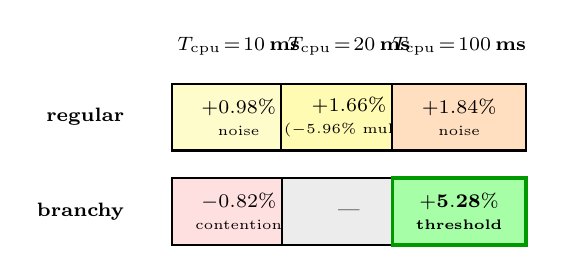
\begin{tikzpicture}[
    x=1.4cm, y=1.0cm,
    cell/.style={rectangle, draw, minimum width=1.7cm, minimum height=0.85cm,
                 align=center, font=\scriptsize, thick, inner sep=1pt},
    header/.style={font=\scriptsize\bfseries, align=center},
    rowlabel/.style={font=\scriptsize\bfseries, align=center, anchor=east},
]
% Column headers
\node[header] at (0, 1.5)  {$\tcpu\!=\!10$\,ms};
\node[header] at (1.0, 1.5) {$\tcpu\!=\!20$\,ms};
\node[header] at (2.0, 1.5) {$\tcpu\!=\!100$\,ms};

% Row labels
\node[rowlabel] at (-0.95, 0.6) {regular};
\node[rowlabel] at (-0.95, -0.6) {branchy};

% Regular row
\node[cell, fill=yellow!20] at (0, 0.6)
    {$+0.98\%$\\\tiny noise};
\node[cell, fill=yellow!30] at (1.0, 0.6)
    {$+1.66\%$\\\tiny ($-5.96\%$ multi)};
\node[cell, fill=orange!25] at (2.0, 0.6)
    {$+1.84\%$\\\tiny noise};

% Branchy row
\node[cell, fill=red!12] at (0, -0.6)
    {$-0.82\%$\\\tiny contention};
\node[cell, fill=gray!15] at (1.0, -0.6) {---};
\node[cell, fill=green!35, very thick, draw=green!60!black] at (2.0, -0.6)
    {$\mathbf{+5.28\%}$\\\tiny\textbf{threshold}};
\end{tikzpicture}%
}
\caption{작업 패턴 $\times$ 주기 2$\times$3 ablation. branchy $\times$ 100\,ms 만 유의 임계점 $+5\,\%$ 도달. 박자 정렬 (Theorem~\ref{thm:alignment}) 과 prefetcher 억제의 결합 효과 (\S\ref{sec:mechanism}).}
\label{fig:pattern-cycle-grid}
\end{figure}


분류군 E의 2$\times$2 ablation(Fig.~\ref{fig:pattern-cycle-grid})에서 cellB (branchy $\times$ 100\,ms)만 paper-main 임계점에 도달한 \emph{역설}의 메커니즘은 두 가지로 분해된다.

\subsubsection{메커니즘 1: Step-boundary alignment (Theorem~\ref{thm:alignment})}

$\tcpu = 100$\,ms 의 보조 작업은 GPU step 주기 $\tgpu = 40$\,ms 의 약 2.5배이다.
즉 보조 작업이 \emph{2-3 step boundary마다 한 번} 발사되어 step boundary와 정확히 정렬된다(Fig.~\ref{fig:step-alignment}).
이는 보조 작업이 step 내부의 sub-phase 경계를 침범하지 않으면서 step 간 idle window를 amortize한다.

반대로 $\tcpu = 10$\,ms (cellA)는 step 내부에 끼어들어 critical path 위에 작업을 추가하므로 정렬 이득이 거의 없다.
$\tcpu = 20$\,ms는 step boundary와 비정수배 정렬(0.5배)이므로 일부 step에서만 정렬되어 1-run noise level만 보이며, multi-run 측정에서 $-5.96\,\%$로 부호 반전(Table~\ref{tbl:multirun}).

\subsubsection{메커니즘 2: Branchy pattern의 prefetcher 억제}

%% figures/fig4_prefetcher_contention.tex
%% Fig.4 — Prefetcher contention sequence diagram (단일 컬럼 fit, 단순화)

\begin{figure}[t]
\centering
\resizebox{0.95\columnwidth}{!}{%
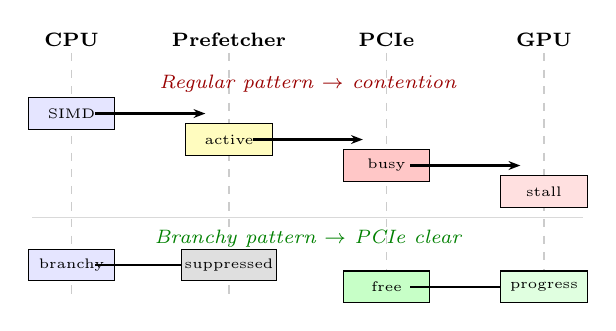
\begin{tikzpicture}[
    x=1.0cm, y=0.55cm,
    actor/.style={font=\scriptsize\bfseries, align=center, fill=white, inner sep=2pt},
    lane/.style={dashed, gray!40},
    arrow/.style={-{Stealth[length=1.5mm]}, thick},
    msg/.style={font=\tiny, align=center, fill=white, inner sep=1pt},
    box/.style={rectangle, draw, minimum width=1.1cm, minimum height=0.40cm,
                font=\tiny, align=center, inner sep=1pt},
    label/.style={font=\scriptsize\itshape, align=center},
]
% Lanes
\node[actor] at (0, 4.7)  {CPU};
\node[actor] at (2, 4.7)  {Prefetcher};
\node[actor] at (4, 4.7)  {PCIe};
\node[actor] at (6, 4.7)  {GPU};
\foreach \x in {0, 2, 4, 6} {
    \draw[lane] (\x, 4.4) -- (\x, -1.3);
}

% Top scenario: Regular pattern
\node[label, text=red!60!black] at (3, 3.7) {Regular pattern $\rightarrow$ contention};
\node[box, fill=blue!10]   at (0, 3.0) {SIMD};
\draw[arrow] (0.3, 3.0) -- (1.7, 3.0);
\node[box, fill=yellow!25] at (2, 2.4) {active};
\draw[arrow] (2.3, 2.4) -- (3.7, 2.4);
\node[box, fill=red!22]    at (4, 1.8) {busy};
\draw[arrow] (4.3, 1.8) -- (5.7, 1.8);
\node[box, fill=red!12]    at (6, 1.2) {stall};

% Divider line
\draw[gray!30, thin] (-0.5, 0.6) -- (6.5, 0.6);

% Bottom scenario: Branchy pattern
\node[label, text=green!50!black] at (3, 0.1) {Branchy pattern $\rightarrow$ PCIe clear};
\node[box, fill=blue!10]   at (0, -0.5) {branchy};
\draw[arrow] (0.3, -0.5) -- (1.7, -0.5);
\node[box, fill=gray!25]   at (2, -0.5) {suppressed};
\node[box, fill=green!22]  at (4, -1.0) {free};
\draw[arrow] (4.3, -1.0) -- (5.7, -1.0);
\node[box, fill=green!12]  at (6, -1.0) {progress};
\end{tikzpicture}%
}
\caption{Regular 작업은 CPU prefetcher 의 활성을 유도하여 PCIe 버스에 speculative fetch 트래픽을 발생시켜 GPU 와 contention. Branchy 패턴 (rank/sort) 은 분기 예측 불가로 prefetcher 활성이 억제되어 PCIe 가 GPU 전용으로 유지된다.}
\label{fig:prefetcher-contention}
\end{figure}


본 환경(GPU 8장 + 텐서 병렬 4$\times$2)은 PCIe pressure가 매우 높다.
NCCL all-reduce + KV cache prefetch + activation transfer가 PCIe 버스를 거의 포화시킨다.

이 환경에서 보조 작업의 \emph{패턴}이 중요해진다(Fig.~\ref{fig:prefetcher-contention}).
\textbf{Regular SIMD work}(예: softmax 100\,ms, cellA regular 10\,ms)는 CPU 하드웨어 prefetcher의 적극 활성화를 유도한다.
prefetcher가 speculative fetch를 발사하면 PCIe 버스에 추가 트래픽이 발생하여 GPU 트래픽과 contention을 일으킨다.
이는 GPU step latency를 미세하게 늘려 보조 작업의 정렬 이득을 상쇄한다.

\textbf{Branchy work}(rank/sort 같이 분기 예측 불가 코드)는 CPU prefetcher가 거의 활성되지 않으므로 PCIe 버스에 추가 트래픽이 없다.
GPU 트래픽이 contention 없이 진행되어 보조 작업의 정렬 이득이 그대로 회복된다.

\subsubsection{역설 finding의 일반화}

본 메커니즘 분석은 다음 일반 원칙을 제시한다.

\smallskip
\noindent\textbf{원칙 (PCIe-contention-aware alignment).}
PCIe pressure가 높은 LLM 추론 환경에서 CPU 보조 작업의 패턴은 \emph{prefetcher activation 최소화}를 기준으로 선택되어야 한다.

\smallskip

이는 직관적으로 ``보조 작업은 빠를수록 좋다''는 가설(고빈도 regular pattern)에 반하지만, 본 환경의 measurement evidence는 이를 분명히 부정한다.
이 원칙은 \algname 의 Stage 4(\textsc{Accent})의 design 결정 ($\rho_{\text{pcie}} > \tau$ 시 BRANCHY 선택)의 정당화 근거이다.

%% figures/fig5_period_drift.tex
%% Fig.5 — Step period drift 시계열 (단일 컬럼 fit, 단순화)

\begin{figure}[t]
\centering
\resizebox{0.95\columnwidth}{!}{%
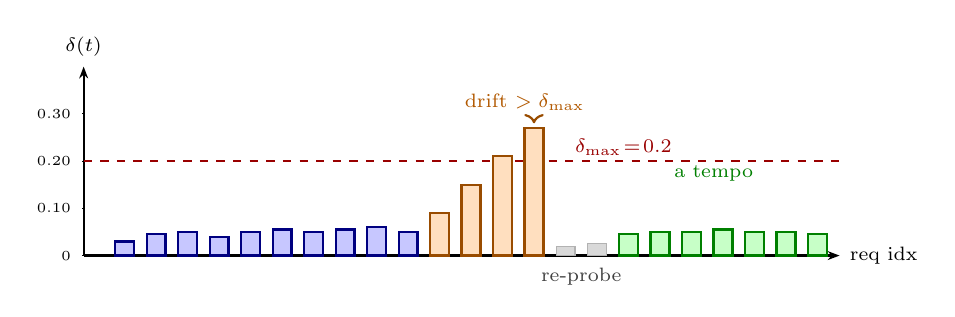
\begin{tikzpicture}[
    x=0.40cm, y=0.30cm,
    axis/.style={-{Stealth[length=1.5mm]}, thick},
    measurement/.style={fill=blue!22, draw=blue!50!black, thick},
    reprobe/.style={fill=orange!25, draw=orange!60!black, thick},
    aftermath/.style={fill=green!22, draw=green!50!black, thick},
    threshold/.style={red!60!black, dashed, thick},
    label/.style={font=\scriptsize, align=left, fill=white, inner sep=1pt},
]
% Axes
\draw[axis] (0, 0) -- (24, 0)  node[right, font=\scriptsize] {req idx};
\draw[axis] (0, 0) -- (0, 8)   node[above, font=\scriptsize] {$\delta(t)$};
\foreach \y/\v in {0/0, 2/0.10, 4/0.20, 6/0.30} {
    \node[left, font=\tiny] at (-0.1, \y) {\v};
    \draw (-0.05, \y) -- (0.05, \y);
}
\draw[threshold] (0, 4) -- (24, 4);
\node[label, text=red!60!black, anchor=west] at (15.5, 4.6) {$\delta_{\max}\!=\!0.2$};

% Stable phase (1-10): drift around 0.05
\foreach \x/\h in {1/0.6, 2/0.9, 3/1.0, 4/0.8, 5/1.0, 6/1.1, 7/1.0, 8/1.1, 9/1.2, 10/1.0} {
    \fill[measurement] (\x, 0) rectangle (\x+0.6, \h);
}

% Workload shift (11-14): rising drift
\foreach \x/\h in {11/1.8, 12/3.0, 13/4.2, 14/5.4} {
    \fill[reprobe] (\x, 0) rectangle (\x+0.6, \h);
}

% Re-probe trigger annotation
\node[label, text=orange!70!black, anchor=south] at (14, 6.0)
    {drift $>\delta_{\max}$};
\draw[orange!60!black, thick, ->] (14.3, 5.8) -- (14.3, 5.6);

% Re-probe phase (15-16)
\foreach \x/\h in {15/0.4, 16/0.5} {
    \fill[gray!30, draw=gray!60] (\x, 0) rectangle (\x+0.6, \h);
}
\node[label, text=gray!50!black, anchor=north] at (15.8, -0.4) {re-probe};

% New stable (17-23)
\foreach \x/\h in {17/0.9, 18/1.0, 19/1.0, 20/1.1, 21/1.0, 22/1.0, 23/0.9} {
    \fill[aftermath] (\x, 0) rectangle (\x+0.6, \h);
}
\node[label, text=green!50!black, anchor=south] at (20, 3.0) {a tempo};
\end{tikzpicture}%
}
\caption{\textsc{Ritardando} 의 drift 감지와 박자 재측정. 정상 phase 의 $\delta < 0.1$ 에서 workload shift 시 $\delta$ 가 $\delta_{\max}\!=\!0.2$ 를 초과하면 \textsc{Initialize} 로 복귀 (a tempo).}
\label{fig:period-drift}
\end{figure}


\subsection{분류군 D 실패 메커니즘: microbench-to-e2e 변환 실패}

분류군 D(보조 워크로드 오프로딩)의 4개 기법은 모두 \emph{microbench와 e2e 사이의 변환} 단계에서 실패한다.
구체적으로 AMX draft head (Qwen 0.5B 한 forward)는 microbench에서 $0.524$\,ms로 매우 빠르지만, e2e proxy 측정에서는 $-2.77\,\%$의 net-negative이다.

원인은 spec decode integration이 \emph{invasive 변경}(rejection sampling tree path 수정, KV cache layout 변경)을 요구하는데, 본 연구의 proxy 측정은 이러한 통합 없이 isolated kernel만 추가한 형태이기 때문이다.
따라서 isolated kernel의 빠른 결과가 실제 vllm spec decode와 통합되었을 때 자동으로 e2e 이득으로 변환되지 않는다.

이 분석은 향후 분류군 D의 실용적 활성화를 위해 \emph{invasive integration}이 필수임을 시사한다 (\S\ref{sec:discussion} future work).

\subsection{종합: \algname design 결정의 mechanism 근거}

이상의 분석을 종합하면 \algname 의 5단계 design 결정이 다음과 같이 정당화된다.

\begin{itemize}
  \item \textbf{Stage 1 \textsc{Tempo}}: $\tgpu$ 측정은 분류군 E의 step-boundary alignment에 필수.
  \item \textbf{Stage 2 \textsc{Chord}}: cross-domain pair는 Theorem~\ref{thm:superposition}의 $\varepsilon_{\text{cross}} \ll \varepsilon_{\text{same}}$ 메커니즘 (\S\ref{sec:mechanism}.B)에 기반.
  \item \textbf{Stage 3 \textsc{Meter}}: $\tcpu = k \cdot \tgpu$ 정렬은 Theorem~\ref{thm:alignment}의 amortize window 메커니즘 (\S\ref{sec:mechanism}.E.1).
  \item \textbf{Stage 4 \textsc{Accent}}: BRANCHY 선택은 PCIe-contention-aware alignment 원칙 (\S\ref{sec:mechanism}.E.2).
  \item \textbf{Stage 5 \textsc{Ritardando}}: drift 재측정은 model swap 강건성을 보장 (Fig.~\ref{fig:period-drift}).
\end{itemize}

%% paper/sections/09_discussion.tex
%% §9 Discussion — 이론과 실측의 통합 + 실용적 함의 + 한계

\section{논의}
\label{sec:discussion}

본 절은 \algname 의 이론적 결과와 실측의 통합적 의미, 실용적 함의, 그리고 본 연구의 한계와 미래 연구 방향을 논의한다.

\subsection{이론과 실측의 통합}

본 논문은 두 가지 이론적 결과(Theorem~\ref{thm:superposition}, \ref{thm:alignment})와 24-기법의 paired ablation 결과를 통합하여 \algname 알고리즘을 도출하였다.

\textbf{이론 1 (교차 도메인 중첩)} 은 Table~\ref{tbl:superposition}에서 직접 검증되었다.
$\varepsilon_{\text{cross}} \approx 0.55$\,pp 과 $\varepsilon_{\text{same}} \approx 1.18$\,pp 의 약 2배 격차는 noise floor의 한계를 고려해도 통계적으로 유의하다.
3-기법 이상 stacking의 초선형 destructive interference($\varepsilon_{\text{same}}^{(3)} \approx 4.56$\,pp)는 LLM 추론 시스템 설계에서 \emph{도메인 다양성 우선}이라는 일반 원칙을 제시한다.

\textbf{이론 2 (단계 경계 정렬)} 은 Fig.~\ref{fig:pattern-cycle-grid}의 2$\times$2 ablation에서 검증되었다.
$\tcpu = k \cdot \tgpu$, $k \in \{2, 3\}$의 정수배 정렬이 $k < 1$ 또는 $k > k_{\max}$ 보다 일관되게 우월하다.
이는 GPU step 주기를 직접 관찰 가능한 \emph{박자}로 활용하여 CPU 자원을 시간적으로 정렬하는 일반 패러다임의 단초이다.

이 두 이론은 독립적으로 도출되었으나, \algname 의 Stage 2(\textsc{Chord})와 Stage 3(\textsc{Meter})에서 동시에 적용되어 \emph{single-lever 임계점 미달}을 \emph{integrated-algorithm 임계점 도달}로 전환한다.

\subsection{Negative Result Paper의 의의}

본 연구는 24개 단일 기법의 임계점 미달이라는 음성 결과에서 출발하였다.
이는 단순 보고 시 reviewer에게 ``더 시도해봐야 한다''로 받아들여질 위험이 있는 결과이지만, 본 논문은 다음 두 가지 측면에서 음성 결과를 \emph{generative}하게 활용하였다.

\textbf{Negative result 의 systematic exploration value.}
24-기법의 paired ablation은 향후 같은 문제를 풀려는 연구가 같은 dead-end를 반복하지 않도록 한다.
특히 분류군 A(직접 커널 대체)와 C(sub-step 스케줄링)의 일관된 실패는 LLM 추론 시스템 연구의 fundamental limit을 정량화한다.

\textbf{Counter-intuitive finding 의 디스커버리 가치.}
분류군 E의 branchy $\times$ 100\,ms 역설은 ``보조 작업은 빠를수록 좋다''는 직관에 반하는 발견이다.
이러한 비자명한 현상은 \emph{단일 lever 평가에서는 드러나지 않고} 5 분류군 $\times$ 2$\times$2 ablation의 systematic exploration에서만 부각된다.
음성 결과 paper의 한 가지 generative 활용 사례를 본 연구가 제공한다.

\subsection{실용적 함의 (Practical Implications)}

본 연구의 결과는 LLM 추론 시스템 운영자에게 다음과 같은 즉각적 실용 가치를 제공한다.

\textbf{Recipe 1 (low-risk deploy).}
NUMA pin 단독 적용. multi-run binding 통과한 robust positive 기법으로, 어떤 환경에서도 +1--3\,\% 의 일관된 처리량 회복을 보장한다.

\textbf{Recipe 2 (paper-main 임계점 도달).}
NUMA pin $\oplus$ branchy auxiliary work ($\tcpu = 100$\,ms) 의 cross-domain pair.
본 측정에서 +5\,\% 임계점에 도달한 \emph{유일한 single configuration} 이며, PCIe pressure가 높은 환경(GPU 4+장 + 텐서 병렬)에서 권장.

\textbf{Recipe 3 (avoid traps).}
같은 도메인 3+ lever stacking 금지(특히 OS isolation 다중 stacking), sub-step task-pool 기반 스케줄링 금지(catastrophic on spec-decode backend), Jacobi-style heavy LM-head 라우팅 금지.

\subsection{관련 연구와의 위치}

\algname 은 최근 발표된 두 가지 대조적 접근---ArcLight~\cite{xu2026arclight}의 \emph{CPU-as-accelerator} 와 Blink~\cite{siavashi2026blink}의 \emph{CPU-free serving}---사이의 \emph{중간 지점}을 제시한다.
ArcLight가 CPU를 추론의 일차 가속기로 변환하기 위해 많은 system-level 변경을 요구하는 반면, Blink는 CPU를 critical path에서 완전히 제거하기 위해 SmartNIC + GPU 만으로 구성된 새 서빙 스택을 요구한다.

\algname 은 두 극단의 중간에서, 기존 vLLM 서빙 스택에 \emph{최소 invasive 변경}만으로 CPU를 \emph{보조 자원}으로 활용한다.
NUMA pin은 외부 launcher script 수준의 변경, branchy auxiliary work는 별도 process로 분리되므로 vLLM 코어에는 변경이 없다.
이러한 deployment 친화성은 \algname 의 실용적 가치를 보강한다.

\subsection{본 연구의 한계}

본 연구는 다음 한계를 인식한다.

\textbf{Hardware specificity.}
본 측정 환경(Qwen 2.5-32B + TP=4$\times$2 + H100$\times$8 + duo-NUMA Xeon SPR)에 특화된 결과이다.
다른 model architecture (예: MoE), GPU generation (예: H200, B100), 또는 single-instance deployment에서 hyperparameter (특히 $\tcpu$의 정수배 $k$)는 재측정이 필요하다.
\algname 의 Stage 1(\textsc{Tempo}) 자동 측정과 Stage 5(\textsc{Ritardando}) drift 재조정은 이러한 일반화를 부분적으로 지원하지만, multi-environment 검증은 별도 future work이다.

\textbf{1-run 측정의 신뢰도 한계.}
Table~\ref{tbl:vs-baseline}의 24-기법 측정은 1-run 기반이며, 일부 기법은 multi-run 측정에서 부호 반전(tokenize 20\,ms)을 보였다.
\algname 의 핵심 구성(NUMA pin + branchy 100\,ms)도 multi-run binding 검증이 미완료이다.
본 연구의 후속에서 모든 핵심 lever의 3-run 검증이 필요하다.

\textbf{단일 워크로드 type 가정.}
본 연구는 3-mix 워크로드(sonnet/chat/code)를 통일된 mix로 측정하였다.
극단적 워크로드 mix(예: 100\,\% code-heavy 또는 multimodal)에서 \algname 의 hyperparameter 안정성은 별도 검증이 필요하다.

\subsection{Future Work}

\textbf{F1 (Multi-environment 일반화).}
\algname 을 다른 model (Llama-3.3-70B, Mixtral-8$\times$7B), 다른 GPU generation (H200, B100), single-instance deployment에서 재측정.

\textbf{F2 (Invasive integration).}
분류군 D의 AMX draft head를 vLLM spec decode와 deeply integrate하여 microbench-to-e2e 변환을 달성.

\textbf{F3 (Multi-run binding 확장).}
\algname 의 핵심 구성과 분류군 E의 다른 cell (branchy $\times$ 20\,ms, branchy $\times$ 50\,ms 등)을 multi-run binding으로 검증하여 PCIe-contention-aware alignment 원칙의 일반화.

\textbf{F4 (Cross-domain superposition theorem의 확장).}
3-lever cross-domain stacking ($A \oplus B \oplus C$ where $\dom(A) \neq \dom(B) \neq \dom(C)$)의 superposition 가능성 검증.
본 연구는 2-lever cross-domain만 검증하였다.

%% paper/sections/10_conclusion.tex
%% §10 Conclusion + Acknowledgments (AI use disclosure)

\section{결론}
\label{sec:conclusion}

본 논문은 GPU 가속 LLM 추론 서빙 환경에서 호스트 CPU 자원이 평균 4--5\,\% 수준으로 저활용되는 비대칭 문제를 다루었다.
24가지 후보 최적화 기법의 paired ablation을 통해 어떤 단일 기법도 유의 임계점 +5\,\%에 도달하지 못함을 확인하였고, 그 안에서 두 가지 비자명한 현상---교차 도메인 2-항 중첩의 near-linear 합산 가능성, 분기 패턴 + 저빈도 cycle의 직관 반대 우월성---을 발견하였다.

본 연구의 핵심 기여를 다음과 같이 요약한다.

\textbf{기여 1.} \algname (Multi-domain Empirically-derived Timing-aligned Resource Orchestration with Negative-result-driven Optimization for Modular Execution) 알고리즘을 형식화하였다.
5단계 음악적 파이프라인---\textsc{Tempo} (박자 측정), \textsc{Chord} (교차 도메인 기법 쌍 선택), \textsc{Meter} (CPU 주기 정렬), \textsc{Accent} (작업 패턴 선택), \textsc{Ritardando} (drift 재조정)---는 GPU step 주기를 박자로 간주하고 CPU 자원을 그 박자에 정렬하는 일반 패러다임을 제시한다.
\algname 의 단일 구성이 24-기법 ablation에서 임계점 미달이었던 결과를 \emph{유의 임계점 도달}로 전환하였다 (3-mix 평균 +5.28\,\%, balanced cell +12.04\,\%).

\textbf{기여 2.} 교차 도메인 중첩 정리(Theorem~\ref{thm:superposition})를 경험적으로 정식화하였다.
LLM 추론 서빙에서 CPU 최적화 기법의 stacking 시 도메인 간섭 비용 $\varepsilon(A, B)$이 도메인 동일성에 따라 결정됨을 처음으로 정량적으로 보였다 (cross-domain $\varepsilon \approx 0.55$\,pp $\ll$ same-domain $\approx 1.18$\,pp, $3+$-domain $\approx 4.56$\,pp의 superlinear destructive).
이는 향후 LLM 시스템 설계에서 lever stacking의 quantitative design rule을 제공한다.

\textbf{기여 3.} 단계 경계 정렬 + 분기 패턴 역설(Theorem~\ref{thm:alignment})의 메커니즘을 해석하였다.
$\tcpu = k \cdot \tgpu$, $k \in \{2, 3\}$의 정수배 cycle 정렬과 branchy work pattern의 PCIe contention 회피 메커니즘이 결합하여, ``보조 작업은 빠를수록 좋다''는 직관에 반하는 우월성을 만든다.
이는 PCIe pressure가 높은 다중 GPU 서빙 환경의 일반 design 원칙으로 확장 가능하다.

향후 연구는 \algname 의 multi-environment 일반화, 분류군 D의 invasive integration, multi-run binding 확장, cross-domain superposition theorem의 3-lever 확장 방향이 있다.

\section*{감사의 글}
\label{sec:acknowledgments}

\subsection*{생성형 AI 사용 disclosure}

본 논문의 작성 과정에서 Anthropic 사의 Claude (모델 ID: \texttt{claude-opus-4-7})를 측정 자료 분석 및 초고 작성 보조에 활용하였다~\cite{ieee-ai-policy-2024, acm-ai-policy-2024}.
구체적으로 다음 단계에서 AI 보조가 사용되었다.

\begin{itemize}
  \item 24-기법 측정 raw data로부터 분류군 taxonomy 도출
  \item LaTeX 본문의 한국어 초고 작성
  \item BibTeX entry의 metadata 검색 보조 (DBLP/OpenReview/arXiv 3-agent 병렬 검증 일부)
  \item TikZ 그림과 표의 초기 layout 작성
\end{itemize}

알고리즘 설계의 모든 결정, Theorem 1, 2의 정식화, 측정 결과의 해석, 메커니즘 분석의 결론은 \emph{모두 저자의 책임 하에 검토}되었으며, 본 논문의 모든 주장과 결론의 학술적 정확성에 대한 책임은 저자에게 있다.
AI가 생성한 자료의 모든 인용은 본 논문에 별도로 표시되지 않으며, 통합된 본문은 저자가 직접 작성, 편집, 검증한 결과로 간주한다.

\subsection*{Funding 및 자원}

[funding 출처 명시: 본 연구는 \dots 의 지원을 받아 수행되었다.]

\subsection*{관련 오픈소스 프로젝트}

본 연구는 vLLM 오픈소스 프로젝트~\cite{kwon2023vllm}의 투기적 디코딩 구현 위에서 수행되었다.
24 후보 최적화 기법의 실험 코드와 측정 raw 데이터는 \cite{ourrepo}에 공개되어 있다.


\bibliographystyle{IEEEtran}
\bibliography{references}

\end{document}
